\documentclass[11pt,twoside]{article}

\usepackage[margin=1in]{geometry}
\usepackage{amsmath,amssymb,amsthm,mathtools}
\usepackage[inline,shortlabels]{enumitem}
\usepackage{graphicx}
\usepackage{tikz}
\usetikzlibrary{arrows.meta,calc,decorations.pathreplacing,positioning}
\usepackage{xcolor}
\usepackage{microtype}

% Revision date: maintained by scripts/build_lecture_notes.py. Keep this command.
\newcommand{\lecturerevised}{2026-09-16 09:57 UTC-06:00}
\usepackage{eso-pic}
\AddToShipoutPictureBG{%
  \AtPageLowerLeft{%
    \put(\LenToUnit{0.5\paperwidth},\LenToUnit{0.5in}){%
      \makebox(0,0){\normalfont\footnotesize\color{black!60}Last revised: \lecturerevised}%
    }%
  }%
}

\usepackage[square,authoryear]{natbib}
\usepackage[colorlinks=true,linkcolor=blue!60!black,urlcolor=blue!60!black,citecolor=blue!60!black]{hyperref}
\usepackage[nameinlink,noabbrev,capitalize]{cleveref}
\crefname{exercise}{Exercise}{Exercises}
\Crefname{exercise}{Exercise}{Exercises}

% Short refinements that may be skipped on a first reading.
\usepackage{enotez}
\DeclareInstance{enotez-list}{lecture}{list}{format=\normalsize,number={#1.}}
\setenotez{list-name=Endnotes,list-style=lecture,backref=true}
\crefname{endnote}{Endnote}{Endnotes}
\Crefname{endnote}{Endnote}{Endnotes}


\definecolor{courseblue}{HTML}{17365D}
\definecolor{diagramaccent}{HTML}{087FB5}
\definecolor{diagramshell}{HTML}{F1F3F5}
\definecolor{diagramgpt}{HTML}{BFD8E8}
\definecolor{diagramllama}{HTML}{AFB5BA}
\definecolor{diagramdark}{HTML}{52697C}
\definecolor{diagraminset}{HTML}{F7F9FA}

\DeclareMathOperator{\softmax}{softmax}
\newcommand{\R}{\mathbb R}
\newcommand{\Hent}{\mathsf H}

\theoremstyle{plain}
\newtheorem{theorem}{Theorem}[section]
\theoremstyle{definition}
\newtheorem{example}{Example}[section]
\theoremstyle{remark}
\newtheorem{remark}{Remark}[section]


\renewcommand{\thepage}{1--\arabic{page}}
\renewcommand{\thesection}{1.\arabic{section}}
\renewcommand{\theequation}{1.\arabic{equation}}

\pagestyle{myheadings}
\markboth{Lecture 1: Decoder transformers and autoregressive inference}
{Lecture 1: Decoder transformers and autoregressive inference}

\usepackage{../exercises/course-exercises}

\begin{document}

\begin{center}
\fcolorbox{courseblue}{white}{%
\begin{minipage}{0.92\textwidth}
\vspace{1mm}
\textbf{CMPUT 654: Mathematical Foundations of Modern AI Systems}
\hfill Fall 2026

\vspace{3mm}
\begin{center}
{\Large\bfseries Lecture 1: Decoder transformers and autoregressive inference}

\vspace{1mm}
September 1, 2026
\end{center}

\vspace{2mm}
\textit{Lecturer: Csaba Szepesv\'ari}
\hfill
\textit{Note prepared by: Csaba Szepesv\'ari}
\vspace{1mm}
\end{minipage}}
\end{center}

\noindent\textbf{About these lecture notes.}
These notes give a self-contained account of inference through an
archetypical decoder-transformer architecture.
They began as an example of a scribe note and have grown to include further
derivations, figures, and background. This extended treatment is not expected
of student scribe submissions; published notes may incorporate additions by
the lecturer.

\medskip
\noindent\textbf{Scope relative to class.}
Administrative material occupied a substantial part of the meeting. The class
covered the harness, tokenization, decoder inference, mixture-of-experts layers,
attention cost, KV caching, and context-length limitations. Training was
discussed verbally, without loss or gradient equations. These notes supply
explicit matrix conventions, multi-head attention and normalization formulas,
and further derivations and figures. The architecture comparison in
\cref{app:transformer-arrangements} and tokenizer construction in
\cref{app:tokenizer-construction} provide optional background. The motivation
for learning and the first learning-theoretic results begin in Lecture~2.
The optional architecture comparison precedes the take-home messages. Numbered
endnotes, bibliographical notes, the glossary, exercises, the tokenizer
appendix, and references follow in that order.

\section{The model inside a harness}

The goal of this lecture is to understand the computation performed by a
decoder transformer and its role in an AI system. We follow the path from a
token prefix to the next-token distribution, then examine generation,
computational cost, and context-length limitations.

As of 2026, today's cutting edge AI systems are composed of a big neural network and some code that makes the neural network usable.
A
\emph{harness} is the surrounding program that constructs the model's context,
calls the model, interprets the result, optionally invokes tools, records the
new observation, and decides whether to call the model again. It may provide
instructions, conversation history, retrieved documents, external memory, or
tool outputs. \Cref{fig:harness-loop} shows the harness loop and the
token-generation loop within a model call.
The \emph{prompt} is the initial input supplied to a model call. After
tokenization, the prompt tokens form the initial prefix; generated tokens then
extend that prefix.
Output tokens may be detokenized into text or parsed as a tool call. The
resulting observation updates the task state, and the loop may begin again. A
harness can use several model calls before returning an answer. The behavior
of the complete system can therefore depend on the tokenizer, model
parameters, decoding rule, maintained state, tools, and control loop. The rest
of this note expands the tokenizer and model boxes.

\clearpage
\begin{figure}[!ht]
\centering
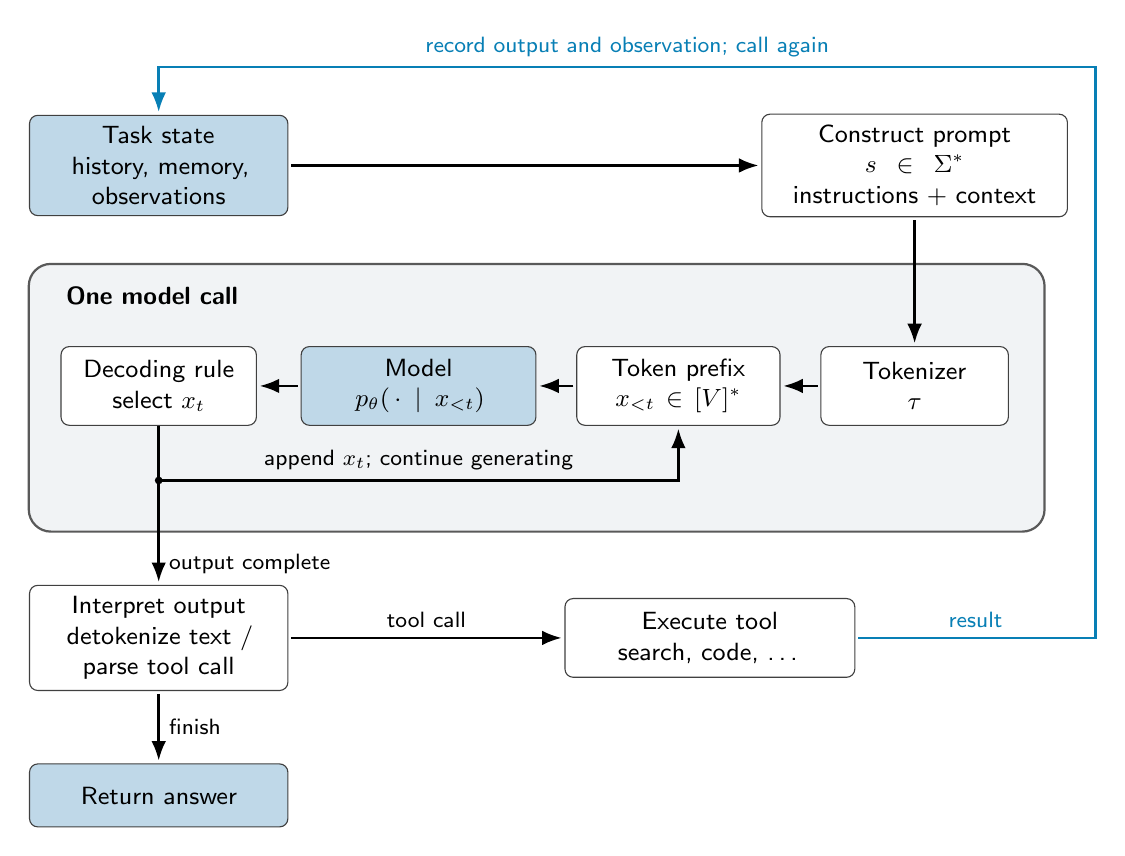
\begin{tikzpicture}[
  harnesspanel/.style={draw=black!65,rounded corners=8pt,fill=diagramshell,
    line width=0.8pt},
  harnessbox/.style={draw=black!75,rounded corners=3pt,fill=white,
    text width=25mm,minimum height=10mm,align=center,
    font=\sffamily\small,inner sep=4pt},
  harnessflow/.style={->,>=Latex,line width=0.9pt,
    shorten <=1pt,shorten >=1pt},
  harnesslabel/.style={font=\sffamily\footnotesize,align=center}
]
  \node[harnessbox,fill=diagramgpt,text width=30mm] (state) at (1.3,0)
    {Task state\\history, memory, observations};
  \node[harnessbox,text width=36mm] (context) at (10.9,0)
    {Construct prompt\\$s\in\Sigma^*$\\instructions + context};
  \draw[harnessflow] (state) -- (context);

  \filldraw[harnesspanel] (-0.35,-4.65) rectangle (12.55,-1.25);
  \node[anchor=west,font=\sffamily\bfseries\small] at (0,-1.65)
    {One model call};
  \node[harnessbox,text width=21mm] (tokenizer) at (10.9,-2.8)
    {Tokenizer\\$\tau$};
  \node[harnessbox,text width=23mm] (prefix) at (7.9,-2.8)
    {Token prefix\\$x_{<t}\in[V]^*$};
  \node[harnessbox,fill=diagramgpt,text width=27mm] (model) at (4.6,-2.8)
    {Model\\$p_\theta(\,\cdot\mid x_{<t})$};
  \node[harnessbox,text width=22mm] (decode) at (1.3,-2.8)
    {Decoding rule\\select $x_t$};
  \draw[harnessflow] (context) -- (tokenizer);
  \draw[harnessflow] (tokenizer) -- (prefix);
  \draw[harnessflow] (prefix) -- (model);
  \draw[harnessflow] (model) -- (decode);
  \coordinate (nextstep) at (1.3,-4.0);
  \draw[line width=0.9pt] (decode.south) -- (nextstep);
  \fill (nextstep) circle (1.4pt);
  \draw[harnessflow] (nextstep)
    -- node[harnesslabel,above] {append $x_t$; continue generating}
    (7.9,-4.0) -- (prefix.south);

  \node[harnessbox,text width=30mm] (interpret) at (1.3,-6.0)
    {Interpret output\\detokenize text /\\parse tool call};
  \draw[harnessflow] (nextstep)
    -- node[harnesslabel,right,pos=0.8] {output complete} (interpret.north);
  \node[harnessbox,text width=34mm] (tool) at (8.3,-6.0)
    {Execute tool\\search, code, \ldots};
  \draw[harnessflow] (interpret)
    -- node[harnesslabel,above] {tool call} (tool);
  \draw[harnessflow,diagramaccent] (tool.east)
    -- node[harnesslabel,above] {result} (13.2,-6.0)
    -- (13.2,1.25)
    -- node[harnesslabel,above] {record output and observation; call again}
    (1.3,1.25) -- (state.north);
  \node[harnessbox,fill=diagramgpt,text width=30mm,minimum height=8mm]
    (answer) at (1.3,-8.0) {Return answer};
  \draw[harnessflow] (interpret)
    -- node[harnesslabel,right] {finish} (answer);
\end{tikzpicture}
\caption{The model inside a harness. Within a call, decoded tokens extend
the prefix until generation stops. The harness interprets the output and
may execute a tool, record its result, and construct another prompt before
returning an answer. The blue feedback path carries the tool observation
back into the maintained task state. The call boundary is schematic: some
interfaces include tool use and further generation within a single model
call. These variations can be convenient; they preserve the basic loop,
so we use this schematic throughout the note.}
\label{fig:harness-loop}
\end{figure}

\section{Tokenization and the modeled sequence}

The word \emph{tokenization} comes from the compiler pipeline. A compiler's
lexer maps a character stream to tokens such as identifiers, numerals, and
operators using a language specification. An LLM tokenizer has the same broad
string-to-sequence interface. Corpus data normally determines its vocabulary
and segmentation rules; a programming-language specification determines a
compiler's lexer.

Let $\Sigma$ be a finite \emph{base alphabet} and let the \emph{vocabulary} $\mathcal V$
consist of $V$ nonempty strings:
\begin{equation}
\mathcal V=\{v_1,\ldots,v_V\}\subset\Sigma^+.
\end{equation}
To give the model a fixed set of token
choices, we segment the text into vocabulary items and represent each by its
index. A \emph{lossless tokenizer} $\tau$ preserves the original text under concatenation:
\begin{equation}
\tau:\Sigma^*\longrightarrow[V]^*,
\qquad
\tau(s)=(x_1,\ldots,x_T),
\qquad
s=v_{x_1}v_{x_2}\cdots v_{x_T}.
\label{eq:tokenizer}
\end{equation}
\emph{Detokenization} concatenates the vocabulary strings. Several token sequences
may concatenate to the same string, so retokenizing a detokenized sequence
need not recover that sequence. Because every vocabulary item is nonempty,
\begin{equation}
|s|=\sum_{t=1}^T|v_{x_t}|\geq T.
\label{eq:token-length}
\end{equation}
Thus tokenization, understood as segmentation over a fixed base alphabet,
cannot increase sequence length and decreases it whenever at least one chosen
token contains more than one base symbol. Normalization, conversion from
Unicode characters to bytes, and the addition of special tokens may change
the sequence before or after this segmentation; those are separate operations.

Practical tokenizers may also normalize text, first split it into coarse
pieces, or begin from bytes to guarantee coverage. Tokens can represent short
words, word stems, syllable-like fragments, or other character sequences;
their boundaries need not have linguistic significance. Tokenization depends
on surrounding text: prepending characters, words, or even a space can change
the segmentation of existing text, rather than simply insert extra tokens.
The extent of this change depends on the tokenizer's boundary rules.
Appendix~\ref{app:tokenizer-construction} describes how tokenizers may be
constructed from a corpus.

For sequence modeling, we augment the vocabulary with special control tokens
and continue to denote its index set by $[V]$.
Once the tokenizer is fixed, a \emph{probabilistic sequence model} $p_\theta$,
with parameters $\theta$, over the token vocabulary $[V]$ is a map
from finite token sequences to probability
distributions over the next token:
\begin{equation}
\begin{aligned}
p_\theta:[V]^*&\longrightarrow\Delta_V,
&x_{<t}&\longmapsto p_\theta(\,\cdot\mid x_{<t}),\\
\Delta_V&:=\left\{p\in[0,1]^V:\sum_{v=1}^V p_v=1\right\}.
\end{aligned}
\label{eq:sequence-model}
\end{equation}
We introduce a special \emph{beginning-of-sequence token}
$x_0=\mathrm{BOS}$ to mark the beginning of a sequence. It serves as the initial
prefix, allowing the same next-token model to specify the first-token
distribution $p_\theta(\,\cdot\mid x_0)$.
We write $x_{<t}=(x_0,\ldots,x_{t-1})$;
$p_\theta(v\mid x_{<t})$ is the probability assigned to token $v$ after this
prefix. Repeatedly drawing from these distributions defines an infinite
\emph{stochastic process} $(X_t)_{t\geq1}$ on $[V]$. The chain rule gives a fixed
prefix's probability by multiplying its successive conditional probabilities:
\begin{equation}
p_\theta(x_{1:T})
=\prod_{t=1}^T p_\theta(x_t\mid x_{<t}).
\label{eq:autoregressive-factorization}
\end{equation}
Since we are interested in modeling probability distributions
over \emph{finite} (as opposed to infinite) token sequences,
we introduce another special token, the \emph{end-of-sequence token} $\mathrm{EOS}$.
The idea is that once the EOS appears, generation stops.
From the infinite process $(X_t)_{t\geq1}$,
we stop at its first EOS occurrence, the \emph{stopping time} $\tau_{\mathrm{EOS}}$:
\begin{equation}
\tau_{\mathrm{EOS}}=\inf\{t\geq1:X_t=\mathrm{EOS}\},
\label{eq:eos-stopping-time}
\end{equation}
with $\tau_{\mathrm{EOS}}=\infty$ if EOS never occurs. For this construction to
define a probability distribution over finite sequences, one needs the
additional constraint that $\Pr(\tau_{\mathrm{EOS}}<\infty)=1$. Deployed systems
additionally enforce a maximum generation length $M$, stopping at
$\min\{\tau_{\mathrm{EOS}},M\}$. This guarantees finite output, potentially
truncating it before the model produces EOS.

\section{Decoder-only transformers as next-token models}

The preceding section defined a probabilistic sequence model as a map from
token prefixes to next-token distributions, \eqref{eq:sequence-model}.
We now describe decoder-only transformers, a class of neural networks that
power many of today's most capable AI systems. Their computations take place
in real vector spaces: the token prefix is first embedded as a sequence of
real vectors, this sequence is transformed through several layers, and a
\emph{readout} converts the last vector into a next-token distribution.

A central design constraint is that the number of trainable parameters is
independent of the input sequence length: the same parameters are reused
across positions and supported sequence lengths. One trained model can thus
handle inputs of different lengths. Since training data are limited, learning
shared operations from examples at many positions can reduce the data needed
for good generalization. This \emph{inductive bias} assumes that similar
computations are useful across positions and lengths.
Longer inputs require more
computation and activation storage, but no additional trainable parameters.

We use an archetypical architecture built by composing a few reusable
functions. Specific architectures vary in their component maps and in how
those maps are arranged.
\emph{Attention} enriches each position's representation by collecting
relevant information from other positions; a \emph{positionwise feed-forward
network} (FFN) combines and transforms the features available at each
position. Normalization and residual addition organize these
operations into blocks. \Cref{fig:modular-transformer} represents the map from
tokens to probabilities as a \emph{computation graph}. Nodes and labels specify
operations and intermediate quantities; arrows show which quantities each
operation needs. An operation can be evaluated once its inputs are available,
and branching reuses a quantity in several computations.

\paragraph{Sequences of activation vectors.}
Throughout the course, every vector is a column vector. We represent a
sequence $(h_1,\ldots,h_T)$ of vectors in $\R^d$ by a matrix $H$ whose rows
store their transposes:
\begin{equation}
H=
\begin{bmatrix}
h_1^\top\\[-1mm]
\vdots\\[-1mm]
h_T^\top
\end{bmatrix}
\in\R^{T\times d},
\qquad h_i=(H_{i,:})^\top.
\label{eq:row-stacking}
\end{equation}
Thus positions run left to right in a sequence display and top to bottom
in a matrix. Columns index feature coordinates.

For a computation local to one position, we reuse the same rule throughout
the sequence. A function $f:\R^d\to\R^r$ therefore has a
\emph{positionwise lift}, denoted by the same symbol:
\begin{equation}
f(H):=
\begin{bmatrix}
f(h_1)^\top\\[-1mm]
\vdots\\[-1mm]
f(h_T)^\top
\end{bmatrix}
\in\R^{T\times r}.
\label{eq:positionwise-lift}
\end{equation}
The same function, with the same parameters, is applied at every position.
It may mix coordinates within a vector, but it does not exchange information
between positions.

\paragraph{Attention and positionwise operations.}
A \emph{normalization map} $N_\nu:\R^d\to\R^d$ has learned parameters $\nu$ and
adjusts the scale of a vector's feature coordinates; some choices also center
them. This makes the following learned update less sensitive to the overall
activation scale. The FFN computes a map $\operatorname{FF}_\psi:\R^d\to\R^d$ with learned
parameters $\psi$. We lift both maps positionwise using
\eqref{eq:positionwise-lift}, keeping their parameters fixed across positions.
LayerNorm and RMSNorm are examples of $N_\nu$;
see \cref{sec:normalization-maps}. Examples of FFN architectures appear in
\cref{sec:positionwise-ffn}.

An \emph{attention head} $\operatorname{Head}_{\eta,M}$ gathers one input-dependent weighted combination
of source information at each position. We first specify its interface:
for each sequence length $T$, it computes a map
\begin{equation}
\operatorname{Head}_{\eta,M}:
\R^{T\times d}\longrightarrow\R^{T\times d_h}.
\label{eq:head-interface}
\end{equation}
Here $\eta$ collects its learned parameters, whose number is independent of
$T$; the same parameters are reused at every position and sequence length.
The output width is $d_h$, and the mask $M$ specifies which source positions
each output position may use.
A causal mask allows position $i$ to use only positions $1,\ldots,i$,
ensuring that a next-token prediction uses only information available in
its prefix.
This interface does not yet specify the computation.
\Cref{sec:one-attention-head} defines a head using just three learned matrices,
with $3dd_h$ parameters in total.

Several heads allow a position to gather different kinds of information in
parallel. An \emph{output projection} $W^O$ combines their retrieved features into an
update at the model width. For $h$ heads, collect their parameters and a
learned output projection~
\endnote{
Following the literature we use the word projection to denote a linear map, even when
this map does not have the properties of a mathematical projection, hoping that
this will not cause confusion. If this difference becomes important, we will point it out.
} as
$\xi=(\eta_1,\ldots,\eta_h,W^O)$, where
$W^O\in\R^{hd_h\times d}$. The \emph{multi-head attention map}
$\operatorname{SelfAttn}_{\xi,M}:\R^{T\times d}\to\R^{T\times d}$ is defined by
\begin{equation}
\operatorname{SelfAttn}_{\xi,M}(U)
=\bigl[
\operatorname{Head}_{\eta_1,M}(U)\mid\cdots\mid
\operatorname{Head}_{\eta_h,M}(U)
\bigr]W^O.
\label{eq:self-attention-map}
\end{equation}
The brackets concatenate the head outputs into a $T\times hd_h$ matrix;
$W^O$ mixes their features and returns to width $d$. Usually $d_h=d/h$,
so $hd_h=d$. The heads receive the same input and mask, with distinct
parameters.
The mask $M$ is prescribed, separate from the learned parameters $\xi$.

\paragraph{Blocks and their composition.}
A block refines the current representation through \emph{residual
connections}: each sublayer adds an update to its input. A near-identity
map then requires only a small update, a useful bias when composing many
layers.

Fix component architectures and a block parameter collection
$\vartheta=(\xi,\psi,\nu_1,\nu_2)$. One \emph{pre-normalized decoder block}
is the function $\mathcal B_{\vartheta,M}:\R^{T\times d}\to\R^{T\times d}$
defined in two steps. First, normalize the input $H$ to control the scale seen
by attention, gather information from the sequence, and add it to the
unnormalized input to obtain $G$:
\begin{equation}
G=H+\operatorname{SelfAttn}_{\xi,M}\bigl(N_{\nu_1}(H)\bigr).
\label{eq:attention-block-diagram}
\end{equation}
Next, the FFN processes these enriched features separately at each position,
again using normalization before the update and a residual addition after it:
\begin{equation}
\mathcal B_{\vartheta,M}(H)=G+\operatorname{FF}_\psi\bigl(N_{\nu_2}(G)\bigr).
\label{eq:mlp-block-diagram}
\end{equation}
Every term has shape $T\times d$, so the updates can be added positionwise.

Repeating blocks lets later attention computations use information gathered and
processed by earlier blocks, allowing a computation to proceed in stages.
Let $H^0$ be the embedded input sequence. A transformer uses $L$ copies
of this block architecture, with parameter collections
$\theta_\ell=(\xi_\ell,\psi_\ell,\nu_{\ell,1},\nu_{\ell,2})$ that generally differ
between layers:
\begin{equation}
H^{\ell+1}=\mathcal B_{\theta_\ell,M}(H^\ell)\,.
\qquad \ell=0,\ldots,L-1,
\label{eq:block-function}
\end{equation}
Alternatively, one can write the computation as the composition of the $L$ underlying maps:
\begin{equation}
H^L=
\bigl(\mathcal B_{\theta_{L-1},M}\circ\cdots\circ
\mathcal B_{\theta_0,M}\bigr)(H^0).
\label{eq:block-composition}
\end{equation}
Each layer has its own trainable parameters $\theta_\ell$, shared across all positions.

We keep parameters explicit in definitions and when distinguishing component
copies. In a calculation or diagram for a fixed block, we may write
\[
\operatorname{SelfAttn}_M=\operatorname{SelfAttn}_{\xi,M},
\qquad \operatorname{FF}=\operatorname{FF}_\psi,
\qquad N_j=N_{\nu_j}\quad(j=1,2).
\]
We may also shorten $\mathcal B_{\vartheta,M}$ to $\mathcal B_M$, or write
$\mathcal B_{\ell,M}$ for $\mathcal B_{\theta_\ell,M}$ when a layer index
identifies the parameters. These abbreviations are used only when the
suppressed parameters are fixed and unambiguous.

For a prefix $x_{<t}$ of length $T=t$, the readout converts the last hidden vector
$h_t^L=(H^L_{t,:})^\top$ into vocabulary scores $z_t\in\R^V$, called
\emph{logits}, and then into
$p_t:=p_\theta(\,\cdot\mid x_{<t})$ by softmax.
A separate decoding rule selects the next token from $p_t$.
Each block reuses its parameters at every position and for every input
sequence, an extensive form of \emph{weight sharing}.

\begin{figure}[!htbp]
\centering
\resizebox{0.98\textwidth}{!}{%
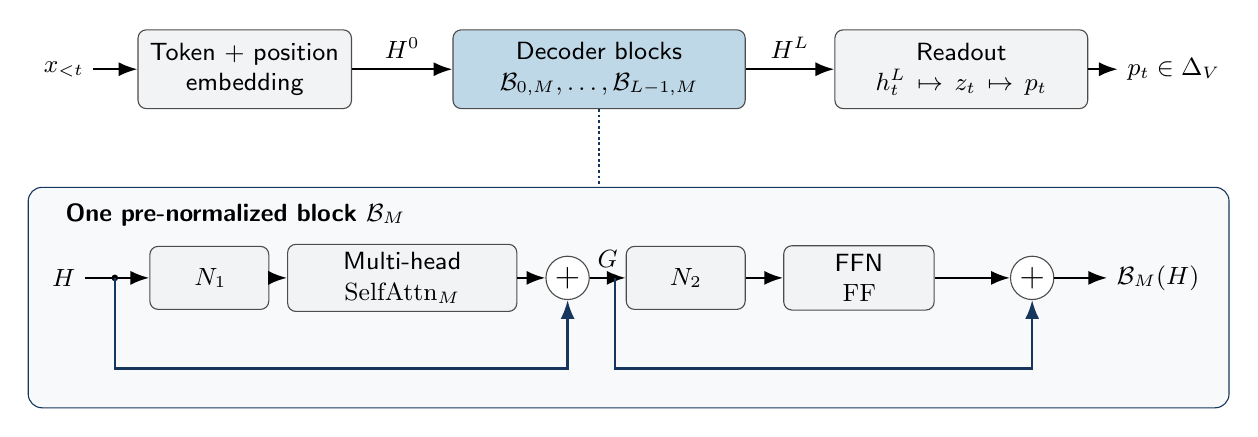
\begin{tikzpicture}[
  module/.style={draw=black!70,rounded corners=3pt,fill=diagramshell,
    text width=25mm,minimum height=10mm,align=center,
    font=\sffamily\small,inner sep=3pt},
  flow/.style={->,>=Latex,line width=0.85pt},
  add/.style={circle,draw=black!70,fill=white,inner sep=0pt,
    minimum size=5.5mm,font=\large},
  lab/.style={font=\small,align=center}
]
\node[lab] (tokens) at (-.3,0) {$x_{<t}$};
\node[module] (embed) at (2.0,0) {Token + position\\embedding};
\node[module,fill=diagramgpt,text width=35mm] (stack) at (6.5,0)
  {Decoder blocks\\$\mathcal B_{0,M},\ldots,\mathcal B_{L-1,M}$};
\node[module,text width=30mm] (readout) at (11.1,0)
  {Readout\\$h_t^L\mapsto z_t\mapsto p_t$};
\node[lab] (prob) at (13.8,0) {$p_t\in\Delta_V$};
\draw[flow] (tokens) -- (embed);
\draw[flow] (embed) -- node[lab,above] {$H^0$} (stack);
\draw[flow] (stack) -- node[lab,above] {$H^L$} (readout);
\draw[flow] (readout) -- (prob);

\filldraw[draw=courseblue,fill=diagraminset,rounded corners=5pt]
  (-.75,-1.5) rectangle (14.5,-4.3);
\node[anchor=west,font=\sffamily\small\bfseries] at (-.4,-1.85)
  {One pre-normalized block $\mathcal B_M$};
\draw[densely dotted,courseblue,line width=1pt]
  (stack.south) -- (6.5,-1.5);
\node[lab] (hin) at (-.3,-2.65) {$H$};
\node[module,text width=13mm,minimum height=8mm] (n1) at (1.55,-2.65)
  {$N_1$};
\node[module,text width=27mm,minimum height=8mm] (att) at (4.0,-2.65)
  {Multi-head\\$\operatorname{SelfAttn}_M$};
\node[add] (plus1) at (6.1,-2.65) {$+$};
\node[module,text width=13mm,minimum height=8mm] (n2) at (7.6,-2.65)
  {$N_2$};
\node[module,text width=17mm,minimum height=8mm] (ff) at (9.8,-2.65)
  {FFN\\$\operatorname{FF}$};
\node[add] (plus2) at (12.0,-2.65) {$+$};
\node[lab] (hout) at (13.6,-2.65) {$\mathcal B_M(H)$};
\draw[flow] (hin) -- (n1);
\draw[flow] (n1) -- (att);
\draw[flow] (att) -- (plus1);
\draw[flow] (plus1) -- node[lab,above] {$G$} (n2);
\draw[flow] (n2) -- (ff);
\draw[flow] (ff) -- (plus2);
\draw[flow] (plus2) -- (hout);
\coordinate (skip1) at (.35,-2.65);
\coordinate (skip2) at (6.7,-2.65);
\fill (skip1) circle (1.2pt);
\fill (skip2) circle (1.2pt);
\draw[flow,courseblue] (skip1) -- (.35,-3.8) -- (6.1,-3.8) -- (plus1.south);
\draw[flow,courseblue] (skip2) -- (6.7,-3.8) -- (12.0,-3.8) -- (plus2.south);
\end{tikzpicture}}
\caption{An archetypical decoder transformer as a composition of maps. A prefix
$x_{<t}$ is embedded as $H^0$, transformed by $L$ decoder blocks, and
read out from the last row of $H^L$ to produce logits $z_t$ and the
next-token distribution $p_t$. The inset expands one block: $N_1,N_2$
are positionwise normalization maps, $\operatorname{SelfAttn}_M$ exchanges
information across positions allowed by mask $M$, and the feed-forward network
(FFN) applies $\operatorname{FF}$ independently at each position. Blue paths
carry the inputs to the two residual additions. All block inputs and outputs
have shape $T\times d$. The labels abbreviate
$\mathcal B_{\ell,M}=\mathcal B_{\theta_\ell,M}$ and suppress the inset's fixed
component parameters. Different blocks may have different parameters; within
a block, parameters are shared across positions and sequence lengths.}
\label{fig:modular-transformer}
\end{figure}

\paragraph{The input embedding.}
The first stage of \cref{fig:modular-transformer} assigns a trainable vector
of features to each token. Learning these vectors lets the model choose a
representation suited to prediction.
Identify token $x_t\in[V]$ with the standard basis vector
$e_{x_t}\in\{0,1\}^V$. For $T$ prediction positions, define
$Z\in\{0,1\}^{T\times V}$ by
\begin{equation}
Z_{t,:}=e_{x_{t-1}}^\top,
\qquad t\in[T].
\end{equation}
Rows of $Z$ index sequence positions and columns index vocabulary items:
$Z_{t,v}=1$ precisely when $x_{t-1}=v$.
An \emph{embedding table} $E\in\R^{V\times d}$ assigns the feature vector
$E^\top e_v=(E_{v,:})^\top$ to token $v$. Multiplying by $Z$ performs the
lookup at every position:
\[
(ZE)_{t,:}=e_{x_{t-1}}^\top E.
\]
Word order also changes meaning: ``the dog bites the man'' and ``the man
bites the dog'' describe different events. We make position information
available to subsequent computations by adding a position vector
$P_{t,:}^\top$ to each token embedding; attention-based alternatives appear in
\cref{sec:attention-position}. Stacking these absolute-position vectors as
rows of $P\in\R^{T\times d}$ gives the input
\begin{equation}
H^0=ZE+P,
\qquad
h_t^0=(H^0_{t,:})^\top
=E^\top e_{x_{t-1}}+P_{t,:}^\top\in\R^d.
\label{eq:input-embedding}
\end{equation}
Rows of $E$ index vocabulary items and columns index model features;
rows of $P$ and $H^0$ store the transposes of position and hidden vectors.\endnote{\textbf{Position information without additive embeddings.}
With $P=0$, $h_t^0=E^\top e_{x_{t-1}}$, so a token has the same input vector
at every position.
The causal mask also carries ordering information through its prefix
restriction, so $P=0$ alone does not make the whole decoder insensitive to order.}\label{rem:position-placement}
The one-hot notation makes the map explicit; an implementation performs a
row lookup in $E$.

Position vectors may be computed by a fixed rule. With learned \emph{absolute
position embeddings}, $P$ consists of the first $T$ rows of a table
$P_{\max}\in\R^{T_{\max}\times d}$, requiring $T\leq T_{\max}$.
This table contributes $T_{\max}d$ parameters, depending on the chosen
maximum context length $T_{\max}$, not the current input length $T$.

The matrix $H^0$ starts the composition in \eqref{eq:block-composition};
\cref{sec:output-readout} specifies its final readout.

\section{The component maps}
\label{sec:component-maps}

We now define the functions used in \cref{fig:modular-transformer}, starting
with the operation that transfers information between positions. A component's
parameters are held fixed while its input sequence varies. Layer indices
are needed only when we assemble different copies of the components and as such
we will suppress them in this section.

\subsection{One attention head}
\label{sec:one-attention-head}

Attention enriches the information available at a sequence position by
collecting information from other positions according to its relevance to
the current position (\cref{fig:attention-head}). For example, in a coding
task, a variable use may need information from its earlier declaration.
We follow one row of the figure, then collect all rows into a matrix
computation.

\begin{figure}[!htbp]
\centering
\resizebox{0.98\textwidth}{!}{%
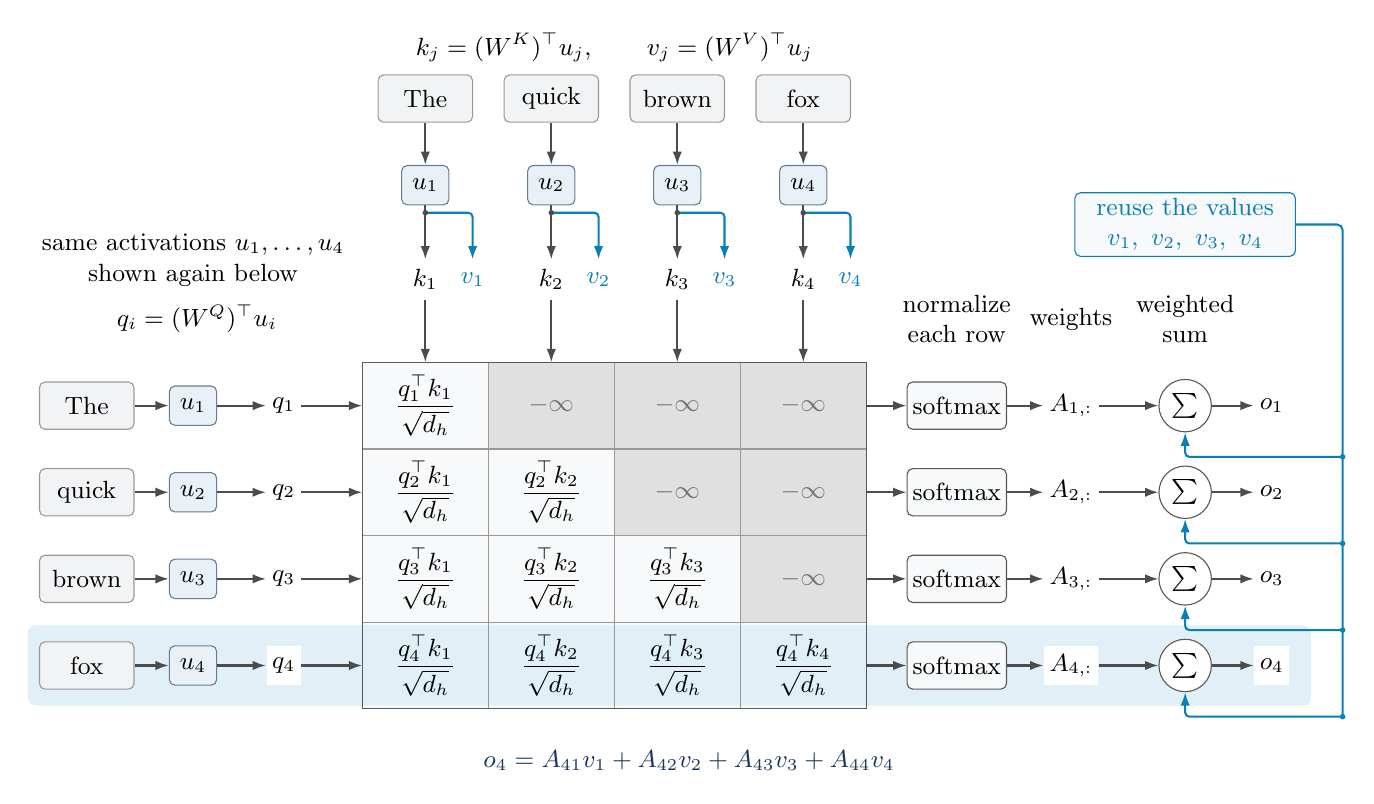
\begin{tikzpicture}[
  font=\small,
  flow/.style={-{Latex[length=1.7mm,width=1.2mm]},line width=.75pt,
    draw=black!70},
  valueflow/.style={-{Latex[length=1.7mm,width=1.2mm]},line width=.75pt,
    draw=diagramaccent,rounded corners=1.5pt},
  lab/.style={align=center,inner sep=2pt},
  token/.style={lab,draw=black!40,fill=diagramshell,rounded corners=2pt,
    minimum width=12mm,minimum height=6mm},
  activation/.style={lab,draw=courseblue!65,fill=diagramgpt!35,
    rounded corners=2pt,minimum width=6mm,minimum height=5mm},
  operation/.style={lab,draw=black!65,fill=diagraminset,rounded corners=2pt,
    minimum height=6mm},
  vector/.style={lab,fill=white,minimum height=5mm}
]
% The grid contains masked scores. Highlight the last query's whole path.
\fill[diagraminset] (0,0) rectangle (6.4,4.4);
\fill[diagramaccent!12,rounded corners=3pt]
  (-4.25,.04) rectangle (12.05,1.06);
\foreach \i in {1,...,4} {
  \foreach \j in {1,...,4} {
    \ifnum\j>\i
      \fill[black!12] ({1.6*(\j-1)},{4.4-1.1*\i})
        rectangle ({1.6*\j},{5.5-1.1*\i});
      \node[lab,text=black!55] at ({1.6*\j-.8},{4.95-1.1*\i})
        {$-\infty$};
    \else
      \node[lab] at ({1.6*\j-.8},{4.95-1.1*\i})
        {$\displaystyle\frac{q_{\i}^{\top}k_{\j}}{\sqrt{d_h}}$};
    \fi
  }
}
\foreach \j in {0,...,4} {
  \draw[black!40,thin] ({1.6*\j},0) -- ({1.6*\j},4.4);
}
\foreach \i in {0,...,4} {
  \draw[black!40,thin] (0,{1.1*\i}) -- (6.4,{1.1*\i});
}
\draw[black!65] (0,0) rectangle (6.4,4.4);

% Each source activation supplies a key for matching and a value to retrieve.
\node[lab] at (3.2,8.4)
  {$k_j=(W^K)^\top u_j,\qquad v_j=(W^V)^\top u_j$};
\foreach \j/\word in {1/The,2/quick,3/brown,4/fox} {
  \node[token] (source-\j) at ({1.6*\j-.8},7.75) {\word};
  \node[activation] (u-\j) at ({1.6*\j-.8},6.65) {$u_{\j}$};
  \node[vector] (k-\j) at ({1.6*\j-.8},5.45) {$k_{\j}$};
  \node[vector,text=diagramaccent] (v-\j)
    at ({1.6*\j-.2},5.45) {$v_{\j}$};
  \draw[flow] (source-\j) -- (u-\j);
  \coordinate (split-\j) at ({1.6*\j-.8},6.3);
  \draw[flow] (u-\j) -- (k-\j);
  \draw[valueflow] (split-\j) -| (v-\j);
  \fill[black!70] (split-\j) circle (1pt);
  \draw[flow] (k-\j) -- ({1.6*\j-.8},4.4);
}

% Repeated activation/value labels denote the same already computed vectors.
\node[lab] at (-2.15,5.7)
  {same activations $u_1,\ldots,u_4$\\shown again below};
\node[lab] at (-2.1,4.95) {$q_i=(W^Q)^\top u_i$};
\node[lab] at (7.55,4.95) {normalize\\each row};
\node[lab] at (9,4.95) {weights};
\node[lab] at (10.45,4.95) {weighted\\sum};
\node[operation,draw=diagramaccent,text=diagramaccent,
  minimum width=28mm] (values) at (10.45,6.15)
  {reuse the values\\$v_1,\ v_2,\ v_3,\ v_4$};
\draw[draw=diagramaccent,line width=.75pt,rounded corners=2pt]
  (values.east) -- (12.45,6.15) -- (12.45,-.1);
\foreach \i/\word in {1/The,2/quick,3/brown,4/fox} {
  \pgfmathsetmacro{\rowy}{4.95-1.1*\i}
  \node[token] (query-token-\i) at (-3.5,\rowy) {\word};
  \node[activation] (query-input-\i) at (-2.15,\rowy) {$u_{\i}$};
  \node[vector] (q-\i) at (-1,\rowy) {$q_{\i}$};
  \draw[flow] (query-token-\i) -- (query-input-\i);
  \draw[flow] (query-input-\i) -- (q-\i);
  \draw[flow] (q-\i) -- (0,\rowy);
  \node[operation] (softmax-\i) at (7.55,\rowy) {softmax};
  \node[vector] (weights-\i) at (9,\rowy) {$A_{\i,:}$};
  \node[circle,draw=black!65,fill=white,inner sep=2pt]
    (sum-\i) at (10.45,\rowy) {$\sum$};
  \node[vector] (out-\i) at (11.55,\rowy) {$o_{\i}$};
  \draw[flow] (6.4,\rowy) -- (softmax-\i);
  \draw[flow] (softmax-\i) -- (weights-\i);
  \draw[flow] (weights-\i) -- (sum-\i);
  \draw[flow] (sum-\i) -- (out-\i);
  \draw[valueflow] (12.45,{\rowy-.65})
    -- (10.45,{\rowy-.65}) -- (sum-\i.south);
  \fill[diagramaccent] (12.45,{\rowy-.65}) circle (1pt);
}
\node[lab,anchor=north,text=courseblue] at (4.15,-.45)
  {$o_4=A_{41}v_1+A_{42}v_2+A_{43}v_3+A_{44}v_4$};
\end{tikzpicture}}
\caption{One causal attention head on ``The quick brown fox,'' assuming one
token per word for illustration (spaces and control tokens are omitted).
Each word labels its position's input activation $u_j$; in deeper layers this
already contains information from earlier positions. Shared projections
compute a key $k_j$, a value $v_j$, and a query $q_j$ at every position.
Matching $u_j$ boxes at the top and left show the same activations;
repeated $v_j$ labels likewise denote reused values. The grid displays
$S+M$: each cell compares its row's query with its column's key; gray cells mask future
positions with $-\infty$. Softmax acts on a whole row, producing weights
$A_{i,:}$ with zeros at masked positions. The sum node uses these weights
and the values supplied by the blue arrows to compute
$o_i=\sum_{j\leq i}A_{ij}v_j$. The highlighted ``fox'' row can retrieve
from all four positions. Keys and values are computed once per position
and reused across queries; the learned matrices $W^Q,W^K,W^V$ are shared
across positions.}
\label{fig:attention-head}
\end{figure}

Let $U\in\R^{T\times d}$ be the input, with activation
$u_i=(U_{i,:})^\top$ at position $i$.

\paragraph{Queries, keys, and values.}
Each input activation vector $u_i$ supplies three vectors: a \emph{query vector} $q_i$ describing
what to look for, a \emph{key vector} $k_i$ used for matching, and a \emph{value vector} $v_i$ containing
what can be retrieved. Separate learned projections $W^Q,W^K,W^V$ let matching and retrieval use
different features. In a coding task, for example, keys might encode variable
names while values carry type information. The head's parameters are
\begin{equation}
\eta=(W^Q,W^K,W^V),
\qquad W^Q,W^K,W^V\in\R^{d\times d_h}.
\label{eq:head-parameters}
\end{equation}
At query position $i$ and source position $j$, these projections give
\[
q_i=(W^Q)^\top u_i,\qquad
k_j=(W^K)^\top u_j,\qquad
v_j=(W^V)^\top u_j
\quad\in\R^{d_h}.
\]
The same activation $u_j$ supplies both $k_j$ and $v_j$; the same projection
matrices are reused at every position. This is \emph{self-attention}:
queries, keys, and values all come from the same input sequence.

\paragraph{Relevance scores.}
A dot product combines matches across feature coordinates into an \emph{attention score}
$S_{ij}$ for source $j$ at query position $i$.
Dividing by the square root of the head width compensates for typical
score growth with width at initialization:
\[
S_{ij}=\frac{q_i^\top k_j}{\sqrt{d_h}}.
\]
Distinct query and key projections allow \emph{directional matching}: the
relevance of one position to another need not be symmetric.
\Cref{rem:attention-scaling} explains the scaling heuristic.

\paragraph{Available positions and weights.}
For autoregressive prediction, the representation predicting $x_i$ must
depend only on $x_{<i}$. During parallel training, later input positions
contain $x_i$ and subsequent tokens, so reading them would reveal the answer.
\emph{Causal attention} enforces the prefix restriction: position $i$ may
use only positions $1,\ldots,i$, excluding future positions.
We enforce this restriction by adding the prescribed \emph{causal mask} $M$ to the scores:
\begin{equation}
M_{ij}=\begin{cases}
0,&j\leq i,\\
-\infty,&j>i.
\end{cases}
\label{eq:causal-mask}
\end{equation}
\emph{Softmax} converts each row's available scores into nonnegative \emph{attention weights} $A_{ij}$
summing to one. Larger scores receive larger weights, while
$e^{-\infty}=0$ removes masked positions:
\[
A_{ij}=
\begin{cases}
\displaystyle\frac{e^{S_{ij}}}{\sum_{r=1}^i e^{S_{ir}}},&j\leq i,\\[2mm]
0,&j>i.
\end{cases}
\]
Its smooth dependence on the finite scores allows gradient-based training.
For \emph{bidirectional attention}, every position can use all $T$ sources:
set $M=0$ and normalize over all of them. Directional matching and causal
masking are separate choices: even without a mask, query--key scores need
not be symmetric.

\paragraph{Collecting the values.}
The weights specify how much information to take from each available
source. Their weighted sum produces the output $o_i$ at position $i$:
\begin{equation}
o_i=\sum_{j=1}^i A_{ij}v_j\in\R^{d_h}.
\label{eq:head-at-one-position}
\end{equation}
Because the weights are nonnegative and sum to one, this is a weighted
average. The highlighted row in \cref{fig:attention-head} shows the case
$i=4$.

\paragraph{All positions at once.}
Stack the transposes of $q_i,k_i,v_i,o_i$ as rows of $Q,K,V,O$.
Their rows index positions and their columns index head features;
in $S$ and $A$, rows index queries and columns index sources.
The following matrix computation summarizes the head and evaluates all
query rows together:
\begin{equation}
\begin{aligned}
Q&=UW^Q,\quad K=UW^K,\quad V=UW^V,
& Q,K,V&\in\R^{T\times d_h},\\
S&=\frac{QK^\top}{\sqrt{d_h}},
& S&\in\R^{T\times T},\\
A&=\softmax_{\mathrm{row}}(S+M),
& A&\in\R^{T\times T},\\
O&=AV,
& O&\in\R^{T\times d_h}.
\end{aligned}
\label{eq:self-attention-heads}
\end{equation}
This defines $\operatorname{Head}_{\eta,M}(U)=O$, with
$o_i=(O_{i,:})^\top$. The $T\times T$ score and weight matrices are
computed activations, not additional parameters. Each key and value is
computed once and reused across query rows; the formulas reuse
$W^Q,W^K,W^V$ at every sequence length.

\begin{remark}[The score-scaling heuristic]
\label{rem:attention-scaling}
Consider a simple random-initialization model. Treat $u_i,u_j$ as fixed
inputs with $\|u_i\|_2^2,\|u_j\|_2^2\approx d$: their mean squared coordinates
are about one, the scale targeted by the normalization examples in
\cref{sec:normalization-maps} before learned rescaling.
Initialize all entries of $W^Q,W^K$ independently with mean zero and
variance $1/d$. This choice keeps projected coordinates at the same scale:
\[
\operatorname{Var}(q_{ir})
=\sum_{a=1}^d u_{ia}^2\operatorname{Var}(W^Q_{ar})
=\frac{\|u_i\|_2^2}{d}\approx1,
\qquad
\operatorname{Var}(k_{jr})=\frac{\|u_j\|_2^2}{d}\approx1.
\]
All variances here concern the random initialization.
The two projections are independent, so $q_{ir}k_{jr}$ has mean zero and
variance $\operatorname{Var}(q_{ir})\operatorname{Var}(k_{jr})\approx1$.
Different coordinates use independent projection columns, making these
products independent across $r$. Summing their variances gives
\[
\operatorname{Var}(q_i^\top k_j)\approx d_h,
\qquad
\operatorname{Var}\!\left(\frac{q_i^\top k_j}{\sqrt{d_h}}\right)\approx1.
\]
The scaling compensates for growth in the initial score variance, helping
avoid overly concentrated softmax weights and small softmax gradients
merely because the head is wider.
Training can change both independence and scale; this argument motivates
the initialization scale without bounding learned scores.
\end{remark}

\begin{remark}[Masks and available source positions]
\label{rem:available-positions}
A mask can equivalently be specified by the positions available to each query.
For every $i\in[T]$, let $\varnothing\ne S_i\subseteq[T]$ be those source
positions. The corresponding matrix mask has $M_{ij}=0$ for $j\in S_i$
and $M_{ij}=-\infty$ otherwise. Given real scores $s_{ij}$ for
$i,j\in[T]$, applying rowwise softmax after adding this mask gives weights $\alpha_{ij}$:
\begin{equation}
\alpha_{ij}=\begin{cases}
\displaystyle\frac{e^{s_{ij}}}{\sum_{r\in S_i}e^{s_{ir}}},&j\in S_i,\\[2mm]
0,&j\notin S_i.
\end{cases}
\label{eq:available-position-attention}
\end{equation}
Thus we can compute attention by summing over available positions directly.
The causal mask uses $S_i=[i]$. For a positive integer width $w$, a
\emph{causal window mask} uses $S_i=\{j\in[i]:i-j<w\}$, retaining only the
most recent $w$ positions, including the query position. Near the start of a
sequence, fewer than $w$ positions are available.
\end{remark}

\subsection{The positionwise feed-forward network}
\label{sec:positionwise-ffn}

The FFN combines and transforms the features available at one position,
including information collected by attention. This lets later attention
heads match using newly computed features, and ultimately helps form the
features used for prediction.
The FFN applies the same learned function $\operatorname{FF}_\psi:\R^d\to\R^d$
independently at each position. Its architecture can be an MLP, a gated
network, or a mixture of experts. We use $\psi$ for its learned parameters.

A \emph{multilayer perceptron} (MLP) is a feed-forward network built from
learned affine maps and coordinatewise activation functions. For a two-layer
example, fix the parameters
\begin{equation}
\begin{gathered}
\psi=(W^1,W^2,b^1,b^2),\\
W^1\in\R^{d\times d_{\rm ff}},\quad
W^2\in\R^{d_{\rm ff}\times d},\quad
b^1\in\R^{d_{\rm ff}},\quad b^2\in\R^d.
\end{gathered}
\label{eq:mlp-parameters}
\end{equation}
For an input $u\in\R^d$, the first affine map forms a vector $a$ of
$d_{\rm ff}$ feature combinations:
\[
a=(W^1)^\top u+b^1\in\R^{d_{\rm ff}}.
\]
A nonlinear \emph{activation function} $\phi:\R\to\R$ transforms these combinations
into hidden features $z$. Nonlinearity matters because composing affine maps
alone would yield another affine map. Apply $\phi$ coordinatewise:
\[
z=\phi(a),\qquad z_r=\phi(a_r).
\]
Common choices include \emph{ReLU}, $\operatorname{ReLU}(s)=\max\{0,s\}$, and
\emph{GELU}, $\operatorname{GELU}(s)=s\Phi(s)$, where $\Phi$ is the standard normal
cumulative distribution function. Finally, a second affine map combines
the new features into an update at the model width:
\begin{equation}
\operatorname{FF}_\psi(u)
= (W^2)^\top z+b^2
= (W^2)^\top\phi\bigl((W^1)^\top u+b^1\bigr)+b^2.
\label{eq:mlp-vector}
\end{equation}
To apply this computation to all positions at once, lift it using
\eqref{eq:positionwise-lift}. Write $\mathbf 1_n\in\R^n$ for the all-ones
column vector; the outer products below copy each bias into every row:
\begin{equation}
\operatorname{FF}_\psi(R)
=\phi\bigl(RW^1+\mathbf 1_T(b^1)^\top\bigr)W^2
+\mathbf 1_T(b^2)^\top,
\qquad R\in\R^{T\times d}.
\label{eq:feed-forward-map}
\end{equation}
For example, row $i$ of $RW^1+\mathbf 1_T(b^1)^\top$ is
$\bigl((W^1)^\top r_i+b^1\bigr)^\top$, where
$r_i=(R_{i,:})^\top$, so the matrix formula applies
\eqref{eq:mlp-vector} independently at each position.

\begin{remark}[Mixture of experts]
\label{rem:moe}
A \emph{mixture-of-experts} (MoE) FFN combines expert maps
$f_1,\ldots,f_m:\R^d\to\R^d$ using input-dependent routing.
A sparse router selects only a few experts to evaluate at each position,
allowing a large collection of learned parameters without using every expert
on every input. For an input $r\in\R^d$, the router selects a small subset $S(r)$ and
nonnegative weights $\rho_e(r)$ summing to one over that subset. Combine
only the selected outputs:
\begin{equation}
f_{\rm MoE}(r)=\sum_{e\in S(r)}\rho_e(r)f_e(r).
\end{equation}
The positionwise lift applies
this same router and expert collection at every position. Here
$\operatorname{FF}_\psi=f_{\rm MoE}$, and $\psi$ collects all expert and router
parameters. This choice of FFN leaves the attention map unchanged.
\end{remark}

\begin{remark}[SwiGLU]
\label{rem:swiglu}
For an input $r\in\R^d$, a \emph{gate} $g(r)$ lets one learned set of features
modulate another, $v(r)$, according to the input.
For \emph{SwiGLU} with hidden width $m$, fix $W_g,W_v\in\R^{m\times d}$ and
$W_o\in\R^{d\times m}$. The projection $W_v$ supplies the features;
$W_g$, followed by the nonlinear \emph{swish} function, supplies the gate:
\[
v(r)=W_vr,\qquad g(r)=\operatorname{swish}(W_gr),\qquad
\operatorname{swish}(s)=\frac{s}{1+e^{-s}},
\]
where swish acts coordinatewise. Multiply each feature by its gate value
using the coordinatewise product $\odot$, defined by $(a\odot b)_i=a_i b_i$,
then combine the products into an output of width $d$:
\begin{equation}
f_{\rm SwiGLU}(r)
=W_o\bigl(g(r)\odot v(r)\bigr)
=W_o\!\left(
\operatorname{swish}(W_g r)\odot (W_v r)
\right).
\end{equation}
Here
$\operatorname{FF}_\psi=f_{\rm SwiGLU}$ and $\psi=(W_g,W_v,W_o)$.
\end{remark}

\subsection{Normalization maps}
\label{sec:normalization-maps}

Successive updates can change the magnitude of a position's activation.
Normalization controls the scale supplied to attention and the FFN, reducing
their sensitivity to such changes.
For a fixed normalization rule, $N_\nu:\R^d\to\R^d$ denotes its map with
learned parameters $\nu$. These parameters are separate from those of
attention and the FFN.

\begin{example}[LayerNorm-type normalization]
\label{rem:rmsnorm}
For an input $u\in\R^d$, first decide whether to remove a common offset
across features. Let $\mu(u)$ be its coordinate mean. A centering choice
$c\in\{0,1\}$ gives the vector $\widetilde u_c$, subtracting the mean when $c=1$:
\[
\mu(u)=\frac1d\sum_{r=1}^d u_r,
\qquad \widetilde u_c=u-c\mu(u)\mathbf 1_d.
\]
Next, form the normalized vector $\widehat u_c$ by dividing by the root
mean square, with a fixed $\varepsilon>0$ to prevent division by zero:
\[
\widehat u_c=
\frac{\widetilde u_c}{\sqrt{d^{-1}\|\widetilde u_c\|_2^2+\varepsilon}}.
\]
Finally, learned scales $\gamma\in\R^d$ and shifts $\beta\in\R^d$ let
the model adjust individual features. The resulting map is
\begin{equation}
N_{c,\gamma,\beta}(u)=\gamma\odot\widehat u_c+\beta
=\gamma\odot
\frac{\widetilde u_c}{\sqrt{d^{-1}\|\widetilde u_c\|_2^2+\varepsilon}}
+\beta.
\label{eq:normalization-family}
\end{equation}
Standard \emph{LayerNorm} centers the features and learns both scale and shift;
\emph{RMSNorm} omits centering and the shift:
\begin{equation}
\operatorname{LayerNorm}_{\gamma,\beta}=N_{1,\gamma,\beta},
\qquad
\operatorname{RMSNorm}_{\gamma}=N_{0,\gamma,0}.
\label{eq:rmsnorm}
\end{equation}
When $c=1$, the denominator uses the coordinate variance; when $c=0$,
it uses the mean square. For LayerNorm, $\nu=(\gamma,\beta)$ and
$N_\nu=N_{1,\gamma,\beta}$. For RMSNorm, which is used in Llama~3,
$\nu=\gamma$ and $N_\nu=N_{0,\gamma,0}$. The centering choice and
$\varepsilon$ are fixed.
\end{example}

The lift in \eqref{eq:positionwise-lift} normalizes each position
separately across its features: $(N_\nu(H)_{i,:})^\top=N_\nu(h_i)$.
Within a fixed block, $N_1=N_{\nu_1}$ and $N_2=N_{\nu_2}$ abbreviate its
two normalization maps, with separate learned parameter collections
$\nu_1,\nu_2$.

\subsection{Layers and shared parameters}

We now assemble copies of these maps in the stack
\eqref{eq:block-composition}. At layer $\ell$, head $a$ has parameters
$\eta_{\ell,a}$, the attention output projection is $W^O_\ell$, the FFN
has parameters $\psi_\ell$, and the normalizations have parameters
$\nu_{\ell,1},\nu_{\ell,2}$. Thus the block's learned parameters are
\begin{equation}
\xi_\ell=(\eta_{\ell,1},\ldots,\eta_{\ell,h},W^O_\ell),
\qquad
\theta_\ell=(\xi_\ell,\psi_\ell,\nu_{\ell,1},\nu_{\ell,2}).
\label{eq:block-parameters}
\end{equation}
Thus layer $\ell$ uses $\operatorname{SelfAttn}_{\xi_\ell,M}$,
$\operatorname{FF}_{\psi_\ell}$, and $N_{\nu_{\ell,1}},N_{\nu_{\ell,2}}$.
The same component formulas apply in every layer, with each layer's own
parameter collection. When the layer index suffices, we may write
$\operatorname{SelfAttn}^{\ell}_M=\operatorname{SelfAttn}_{\xi_\ell,M}$ and
$\operatorname{FF}^{\ell}=\operatorname{FF}_{\psi_\ell}$.

\Cref{fig:parameter-reuse} expands the block graph in
\cref{fig:modular-transformer} across four positions and two layers.
Let $g_i^\ell$ be the vector at position $i$ after the attention residual
update: it is the transpose of row $i$ of $G$ in
\eqref{eq:attention-block-diagram}, applied at layer $\ell$. The operation
nodes compute
\[
g_i^\ell=\mathcal A_{\ell,i}(h_1^\ell,\ldots,h_i^\ell),
\qquad
h_i^{\ell+1}=\mathcal F_{\ell,i}(g_i^\ell).
\]
Here $\mathcal A_{\ell,i}$ includes multi-head attention, the first
normalization, and the first residual update; $\mathcal F_{\ell,i}$ includes
the FFN, second normalization, and second residual update from
\eqref{eq:mlp-block-diagram}. Their parameter collections are
\[
\vartheta_{\ell,1}
=(\xi_\ell,\nu_{\ell,1}),
\qquad
\vartheta_{\ell,2}=(\psi_\ell,\nu_{\ell,2}).
\]
Solid arrows show the causal dependencies: $\mathcal A_{\ell,i}$ reads
positions $1,\ldots,i$, while $\mathcal F_{\ell,i}$ reads only $g_i^\ell$.
Dashed blue branches show reuse of one parameter collection across positions.
Adding positions adds computation nodes and activations, with no new
parameter collections.

\begin{figure}[!htbp]
\centering
\resizebox{0.91\textwidth}{!}{%
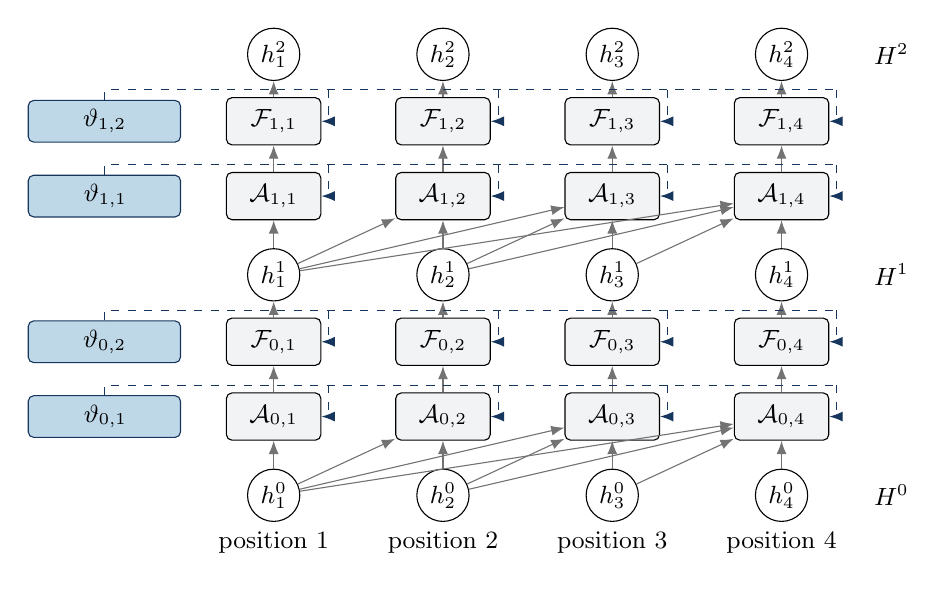
\begin{tikzpicture}[>=Latex,
 act/.style={circle,draw,fill=white,inner sep=2pt,font=\small},
 op/.style={draw,rounded corners=2pt,fill=diagramshell,minimum width=12mm,
 minimum height=6mm,font=\small},
 par/.style={draw=courseblue,fill=diagramgpt,rounded corners=2pt,
 text width=17mm,align=center,font=\small},
 flow/.style={->,black!55,thin},
 reuse/.style={->,dashed,courseblue,thin},
 stage/.style={font=\small,anchor=west}]
\foreach \i in {1,...,4} {
 \node[act] (h0\i) at ({2.15*\i},0) {$h^0_\i$};
 \node[font=\small] at ({2.15*\i},-.6) {position \i};
}
\node[stage] at (9.65,0) {$H^0$};
\foreach \l/\nextlayer/\base in {0/1/0,1/2/2.8} {
 \node[par] (pa\l) at (0,{\base+1.0}) {$\vartheta_{\l,1}$};
 \node[par] (pf\l) at (0,{\base+1.95}) {$\vartheta_{\l,2}$};
 \foreach \i in {1,...,4} {
  \node[op] (a\l\i) at ({2.15*\i},{\base+1.0}) {$\mathcal A_{\l,\i}$};
  \node[op] (f\l\i) at ({2.15*\i},{\base+1.95}) {$\mathcal F_{\l,\i}$};
  \node[act] (h\nextlayer\i) at ({2.15*\i},{\base+2.8}) {$h^{\nextlayer}_\i$};
  \draw[flow] (a\l\i) -- (f\l\i);
  \draw[flow] (f\l\i) -- (h\nextlayer\i);
  \foreach \j in {1,...,\i} {
   \draw[flow] (h\l\j) -- (a\l\i);
  }
 }
 \draw[dashed,courseblue] (pa\l.north) -- (0,{\base+1.4}) -- (9.3,{\base+1.4});
 \draw[dashed,courseblue] (pf\l.north) -- (0,{\base+2.35}) -- (9.3,{\base+2.35});
 \foreach \i in {1,...,4} {
  \draw[reuse] ({2.15*\i+.7},{\base+1.4}) |- (a\l\i.east);
  \draw[reuse] ({2.15*\i+.7},{\base+2.35}) |- (f\l\i.east);
 }
 \node[stage] at (9.65,{\base+2.8}) {$H^{\nextlayer}$};
}
\end{tikzpicture}}
\caption{The block graph of \cref{fig:modular-transformer} expanded across
four positions and two layers, read bottom to top. Circles are vectors
$h_i^\ell$; their transposes form the rows of $H^\ell$.
$\mathcal A_{\ell,i}$ computes causal multi-head attention and its residual
update at position $i$, including the first normalization; its output is
$g_i^\ell$. Each head inside this operation follows \cref{fig:attention-head}.
$\mathcal F_{\ell,i}$ normalizes $g_i^\ell$, applies the FFN, and adds the
result to $g_i^\ell$, producing $h_i^{\ell+1}$.
Solid arrows carry activations. Dashed blue
branches supply one shared parameter collection $\vartheta_{\ell,1}$
or $\vartheta_{\ell,2}$ to all positions in its sublayer.
Crossings are not junctions. Attention heads and intermediate vectors are
suppressed.}
\label{fig:parameter-reuse}
\end{figure}

\begin{remark}[Shared parameters and changing activations]
\label{rem:parameter-reuse}
Within one head, $q_i=(W^Q)^\top u_i$ uses the same matrix at every
position. The FFN and normalization likewise reuse their parameters across
positions. Activations depend on the input and position; longer
sequences require more computation and activation storage while reusing the
same block parameters.
\end{remark}

Causal attention uses only preceding and current positions, and all other
block operations act positionwise. Consequently, after every layer the
vector $h_t^\ell$ depends only on the token prefix $x_{<t}$.
\Cref{app:transformer-arrangements} uses the block notation to compare
encoder-only, decoder-only, and encoder--decoder architectures.

\subsection{Position mechanisms inside attention}
\label{sec:attention-position}
\label{rem:attention-position}

A query may need the value three positions back, or a content match among
nearby positions. Positional mechanisms let attention express such preferences.
For one head, a \emph{relative-position bias} matrix $B$ assigns an additive
preference to each displacement $i-j$. A function $\rho$ clips or buckets
the displacement, and $b$ assigns a learned scalar to each bucket:
\begin{equation}
A=\softmax_{\mathrm{row}}\!\left(
\frac{QK^\top}{\sqrt{d_h}}+M+B
\right),
\qquad
(B)_{ij}=b\bigl(\rho(i-j)\bigr).
\label{eq:relative-position-bias}
\end{equation}
Rows index query
positions and columns index key positions, so $i-j$ compares output position
$i$ with source position $j$. T5 uses this form with the bias parameters
shared across layers and different across heads. ALiBi uses a fixed,
head-dependent linear penalty such as $-m(i-j)$ for a causal pair $j\leq i$.
\emph{Rotary position embeddings} (RoPE) modify the attention calculation by applying position-dependent linear
transformations---specifically, rotations---to the query and key vectors before
taking their inner product.
The query--key dot product then depends explicitly on
the displacement between their positions (see
\cref{ex:rope} for details).

\paragraph{Choosing the frequencies.}
For head width $d_h=2m$, coordinate pair $r\in[m]$ rotates through
$i\omega_r$ radians at position $i$. Its \emph{angular frequency} $\omega_r$
is the angle added per position; we call it simply a \emph{frequency}.
Standard RoPE fixes a geometric schedule:
\begin{equation}
\omega_r=b_{\rm RoPE}^{-(r-1)/m},\qquad r\in[m],\qquad b_{\rm RoPE}>1.
\label{eq:rope-frequencies}
\end{equation}
The original base was $b_{\rm RoPE}=10{,}000$. Fast rotations help distinguish
nearby offsets; slow ones support content comparisons stable over longer
distances. Increasing the base slows rotations for $r>1$, trading local
resolution for stability over longer distances.

\paragraph{What does RoPE learn, and what repeats?}
\label{rem:rope-retrieval}
Training learns the query and key projections. The projected vectors'
magnitudes and relative directions control each frequency's contribution to
the score. Contributions can reinforce one another at a desired displacement
and disagree elsewhere. Because queries and keys depend on the input, these
preferences can depend on content; separate heads learn separate comparisons.
Applying the rotations costs linear work in the head dimension.

One frequency gives periodic dependence on displacement, with a possibly
noninteger period. Combining frequencies can avoid short repetitions, but
distant displacements can still have similar rotations, so long-context
retrieval is not guaranteed. RoPE also does not enforce locality: prescribed
causal and \emph{window masks} exclude future and distant positions,
respectively, as in Mistral~7B.
\Cref{ex:rope} examines retrieval and periodicity; the bibliographical notes
discuss trained models.

\subsection{Architecture examples}

Figures~\ref{fig:gpt2xl} and~\ref{fig:llama3} instantiate our modular
calculation for two dense decoder-only models with different normalization,
FFNs, attention heads, and position mechanisms. They show the full residual
paths and operation placement, including dropout. Numerical labels give
architectural dimensions, not input-dependent activation shapes.

\tikzset{
  archflow/.style={->,line width=0.9pt,>=Latex},
  archskip/.style={->,line width=0.9pt,>=Latex,black!85},
  archleader/.style={densely dotted,line width=1.05pt,diagramdark},
  archbox/.style={draw=black!80,line width=0.75pt,rounded corners=3pt,
    fill=white,minimum height=6.2mm,text width=42mm,align=center,
    inner xsep=2mm,inner ysep=0.7mm,font=\sffamily\small},
  archblockbox/.style={archbox,text width=37mm},
  archsmallbox/.style={archbox,text width=31mm,minimum height=6mm},
  archattention/.style={archblockbox,fill=diagramdark,text=white,
    minimum height=9.2mm},
  archmodule/.style={archblockbox,fill=white!65!diagramgpt},
  archadd/.style={circle,draw=black!80,line width=0.8pt,fill=white,
    inner sep=0pt,minimum size=5.6mm,font=\sffamily\bfseries\large},
  archmult/.style={archadd,minimum size=7mm},
  archfact/.style={align=left,text width=43mm,font=\sffamily\small},
  archcount/.style={font=\sffamily\bfseries\Large,diagramaccent},
  archtitle/.style={font=\sffamily\bfseries\Huge}
}

\begin{figure}[p]
\centering
\resizebox{0.98\textwidth}{!}{%
\begin{tikzpicture}[font=\sffamily]
  \filldraw[rounded corners=12pt,fill=diagramshell,draw=black!70,line width=0.9pt]
    (0.95,1.15) rectangle (9.45,18.75);
  \filldraw[rounded corners=11pt,fill=diagramgpt,draw=diagramdark,
    line width=0.9pt] (2.80,4.70) rectangle (8.15,15.48);

  \node[archtitle] at (5.35,19.55) {GPT-2 XL (1.5B)};

  \node[archsmallbox] (ginput) at (5.35,0.55) {tokenized text};
  \node[font=\ttfamily\small] at (5.35,-0.55) {Every effort moves you};
  \node[archbox] (gembed) at (5.35,1.95) {token embedding layer};
  \node[archbox] (gpos) at (5.35,2.95) {positional embedding layer};
  \node[archbox] (gdrop0) at (5.35,4.05) {dropout};

  \node[archblockbox] (gln1) at (5.35,5.45) {LayerNorm 1};
  \node[archattention] (gatt) at (5.35,6.95)
    {masked multi-head attention};
  \node[archblockbox] (gdrop1) at (5.35,8.45) {dropout};
  \node[archadd] (gadd1) at (5.35,9.51) {$+$};
  \node[archblockbox] (gln2) at (5.35,11.05) {LayerNorm 2};
  \node[archmodule] (gffn) at (5.35,12.55) {FFN};
  \node[archblockbox] (gdrop2) at (5.35,14.05) {dropout};
  \node[archadd] (gadd2) at (5.35,15.35) {$+$};

  \node[archbox] (gfinal) at (5.35,16.55) {final LayerNorm};
  \node[archbox] (gout) at (5.35,17.75) {linear output layer};

  \draw[archflow] (5.35,-0.30) -- (ginput.south);
  \draw[archflow] (ginput) -- (gembed);
  \draw[archflow] (gembed) -- (gpos);
  \draw[archflow] (gpos) -- (gdrop0);
  \draw[archflow] (gln1) -- (gatt);
  \draw[archflow] (gatt) -- (gdrop1);
  \draw[archflow] (gdrop1) -- (gadd1);
  \coordinate (gblockin) at (5.35,4.88);
  \coordinate (gbranch1) at ($(gadd1.north)!0.5!(gln2.south)$);
  \draw[archskip] (gblockin) -- (7.80,4.88)
    -- (7.80,9.51) -- (gadd1.east);
  \draw[archskip] (gbranch1) -- (7.80,10.29)
    -- (7.80,15.35) -- (gadd2.east);
  \draw[archflow] (gdrop0) -- (gln1);
  \draw[archflow] (gadd1) -- (gln2);
  \draw[archflow] (gln2) -- (gffn);
  \draw[archflow] (gffn) -- (gdrop2);
  \draw[archflow] (gdrop2) -- (gadd2);
  \draw[archflow] (gadd2) -- (gfinal);
  \draw[archflow] (gfinal) -- (gout);
  \draw[archflow] (gout) -- (5.35,18.50)
    node[midway,left,font=\sffamily\small] {logits $z_t\in\R^{50{,}257}$};

  \node[rotate=30,inner sep=0pt] at (2.33,5.05)
    {\scalebox{1.30}[2.10]{\Huge$\boldsymbol{\lbrace}$}};
  \node[archcount,anchor=east] at (2.38,4.30)
    {\textbf{48}\,\(\boldsymbol{\times}\)};

  \filldraw[rounded corners=9pt,fill=diagraminset,draw=diagramdark,
    dash pattern=on 2.5pt off 2pt,line width=0.9pt]
    (10.35,10.35) rectangle (15.80,15.85);
  \node[archsmallbox] (gff1) at (13.08,11.25) {linear layer};
  \node[archsmallbox] (ggelu) at (13.08,12.75) {GELU activation};
  \node[archsmallbox] (gff2) at (13.08,14.25) {linear layer};
  \draw[archflow] (gff1) -- (ggelu);
  \draw[archflow] (ggelu) -- (gff2);
  \draw[archleader] (gffn.east) -- (10.35,12.55);

  \node[archfact,anchor=west] (gvocab) at (10.15,18.15)
    {\textbf{Vocabulary size of }
     {\color{diagramaccent}\bfseries 50,257}};
  \draw[archleader] (gout.north east) -- (gvocab.west);

  \node[archfact,anchor=west] (gheads) at (10.15,7.85)
    {{\color{diagramaccent}\bfseries 25} \textbf{heads}};
  \draw[archleader] (gatt.east) -- (gheads.west);

  \node[archfact,anchor=north] (gwidthff) at (13.08,9.45)
    {\textbf{Hidden layer}\\
     \textbf{dimension of }{\color{diagramaccent}\bfseries 6,400}};
  \draw[archleader] (gff1.south) -- (gwidthff.north);

  \node[archfact,anchor=west,text width=50mm] (gcontext) at (10.15,3.35)
    {\textbf{Supported context}\\
     \textbf{length of }{\color{diagramaccent}\bfseries 1,024}\\
     \textbf{tokens with}\\
     \textbf{absolute position}\\
     \textbf{embeddings}};
  \draw[archleader] (gpos.east) -- (gcontext.west);

  \node[archfact,anchor=west] (gwidth) at (10.15,1.55)
    {\textbf{Embedding}\\
     \textbf{dimension of }{\color{diagramaccent}\bfseries 1,600}};
  \draw[archleader] (gembed.east) -- (gwidth.west);

  \node[archfact,anchor=east,text width=31mm] (gcontextshort) at (0.95,2.15)
    {\textbf{Supported}\\
     \textbf{context length}\\
     \textbf{of }{\color{diagramaccent}\bfseries 1024}\textbf{ tokens}};
  \draw[archleader] (gcontextshort.east) -- (gpos.west);
\end{tikzpicture}%
}
\caption{The GPT-2 XL decoder stack. The central blue region is one
pre-normalized transformer block, repeated 48 times; the two side paths are
its residual connections. The inset expands the feed-forward network (FFN),
a two-layer MLP, into its two affine maps and GELU activation.}
\label{fig:gpt2xl}
\end{figure}

\begin{figure}[p]
\centering
\resizebox{0.98\textwidth}{!}{%
\begin{tikzpicture}[font=\sffamily]
  \filldraw[rounded corners=12pt,fill=diagramshell,draw=black!70,line width=0.9pt]
    (1.35,1.15) rectangle (9.55,18.10);
  \filldraw[rounded corners=11pt,fill=diagramllama,draw=black!65,
    line width=0.9pt] (3.00,3.40) rectangle (8.25,13.65);

  \node[archtitle,diagramaccent] at (5.60,18.95) {Llama 3 (8B)};

  \node[archsmallbox] (linput) at (5.60,0.55) {tokenized text};
  \node[font=\ttfamily\small] at (5.60,-0.55) {sample input text};
  \node[archbox] (lembed) at (5.60,2.15) {token embedding layer};

  \node[archblockbox] (lrms1) at (5.60,4.45) {RMSNorm 1};
  \node[archattention] (lgqa) at (5.60,6.10)
    {masked grouped-query attention};
  \node[archadd] (ladd1) at (5.60,7.45) {$+$};
  \node[archblockbox] (lrms2) at (5.60,9.25) {RMSNorm 2};
  \node[archmodule,fill=white!50!diagramllama] (lffn) at (5.60,10.90)
    {FFN};
  \node[archadd] (ladd2) at (5.60,12.60) {$+$};

  \node[archbox] (lfinal) at (5.60,15.05) {final RMSNorm};
  \node[archbox] (lout) at (5.60,16.40) {linear output layer};
  \node[archsmallbox] (lrope) at (0.70,6.10) {RoPE};

  \draw[archflow] (5.60,-0.30) -- (linput.south);
  \draw[archflow] (linput) -- (lembed);
  \draw[archflow] (lrms1) -- (lgqa);
  \draw[archflow] (lrope) -- (lgqa.west);
  \draw[archflow] (lgqa) -- (ladd1);
  \coordinate (lblockin) at ($(lembed.north)!0.68!(lrms1.south)$);
  \coordinate (lbranch1) at ($(ladd1.north)!0.5!(lrms2.south)$);
  \draw[archskip] (lblockin) -- (8.00,3.60)
    -- (8.00,7.45) -- (ladd1.east);
  \draw[archskip] (lbranch1) -- (8.00,8.36)
    -- (8.00,12.60) -- (ladd2.east);
  \draw[archflow] (lembed) -- (lrms1);
  \draw[archflow] (ladd1) -- (lrms2);
  \draw[archflow] (lrms2) -- (lffn);
  \draw[archflow] (lffn) -- (ladd2);
  \draw[archflow] (ladd2) -- (lfinal);
  \draw[archflow] (lfinal) -- (lout);
  \draw[archflow] (lout) -- (5.60,17.85)
    node[midway,left,font=\sffamily\small] {logits $z_t\in\R^{128{,}256}$};

  \node[rotate=30,inner sep=0pt] at (2.66,3.95)
    {\scalebox{1.30}[2.10]{\Huge$\boldsymbol{\lbrace}$}};
  \node[archcount,anchor=east] at (2.68,3.30)
    {\textbf{32}\,\(\boldsymbol{\times}\)};

  \filldraw[rounded corners=9pt,fill=diagraminset,draw=diagramdark,
    dash pattern=on 2.5pt off 2pt,line width=0.9pt]
    (10.10,9.50) rectangle (15.95,15.20);
  \coordinate (lffinput) at (13.00,9.85);
  \node[archsmallbox,text width=21mm] (lgate) at (11.65,10.80)
    {linear layer};
  \node[archsmallbox,text width=21mm] (lvalue) at (14.45,10.80)
    {linear layer};
  \node[archsmallbox,text width=25mm] (lsilu) at (11.65,12.35)
    {SiLU activation};
  \node[archmult] (lmult) at (13.15,13.45) {$\times$};
  \node[archsmallbox] (lproj) at (13.15,14.40) {linear layer};
  \draw[line width=0.9pt] (13.00,9.52) -- (lffinput);
  \draw[archflow] (lffinput) -| (lgate.south);
  \draw[archflow] (lffinput) -| (lvalue.south);
  \draw[archflow] (lgate) -- (lsilu);
  \draw[archflow] (lsilu.north) |- (lmult.west);
  \draw[archflow] (lvalue.north) |- (lmult.east);
  \draw[archflow] (lmult) -- (lproj);
  \draw[archleader] (lffn.east) -- (10.10,10.90);

  \node[anchor=west,align=left,font=\sffamily\small] (lvocab) at (10.10,17.15)
    {\textbf{Vocabulary size of }
     {\color{diagramaccent}\bfseries 128k}\\[-0.3ex]
     \textbf{(128,256)}};
  \draw[archleader] (lout.north east) -- (lvocab.west);

  \node[archfact,anchor=west] (lheads) at (10.10,7.10)
    {{\color{diagramaccent}\bfseries 32} \textbf{heads}};
  \draw[archleader] (lgqa.east) -- (lheads.west);

  \node[archfact,anchor=north west,text width=33mm] (lwidthff) at (10.55,8.75)
    {\textbf{Hidden layer}\\
     \textbf{dimension of }{\color{diagramaccent}\bfseries 14,336}};
  \draw[archleader] ($(lgate.south west)+(0.15,0)$)
    -- (lwidthff.north west);

  \node[archfact,anchor=east,text width=31mm] (lcontext) at (1.25,3.15)
    {\textbf{Supported}\\
     \textbf{context length}\\
     \textbf{of }{\color{diagramaccent}\bfseries 8192}\textbf{ tokens}};
  \draw[archleader] (lcontext.north) -- (lrope.south);

  \node[archfact,anchor=west] (lwidth) at (10.10,2.15)
    {\textbf{Embedding}\\
     \textbf{dimension of }{\color{diagramaccent}\bfseries 4,096}};
  \draw[archleader] (lembed.east) -- (lwidth.west);
\end{tikzpicture}%
}
\caption{The Llama~3 8B decoder stack. The central gray region is one
pre-normalized transformer block, repeated 32 times. RoPE modifies the query
and key vectors inside grouped-query attention. The inset expands the
feed-forward network (FFN), showing both SwiGLU branches, their coordinatewise
product, and the output projection. The 32 attention heads are query heads,
grouped over 8 key/value heads.}
\label{fig:llama3}
\end{figure}
\clearpage

\subsection{Composing attention computations}
\label{sec:composing-attention}

An addressing rule may involve several conditions. For example, in a coding
task, we might want to find an earlier occurrence of an
identifier in the same scope and retrieve its associated value. This requires
representing the identifier and scope, comparing candidate sources, and
retrieving information from a suitable match. How could the components of a
transformer divide this work?

Within one head, the query--key dot product adds contributions from vector
components. If different groups of components represent identifier agreement
and scope agreement, their contributions can jointly favor sources satisfying
both conditions. The representations and score margins must make a joint
match beat a partial match. The positionwise FFNs can transform
and combine features to prepare them for such comparisons in later layers.

Different heads have separate attention distributions and can retrieve
different information in parallel. Their outputs are then combined. Retrieving
an identifier match in one head and a scope match in another, however, does
not establish that the same source satisfies both conditions. A computation
requiring that conjunction must test the conditions together or retain enough
information to check that the retrieved sources coincide.

Layers allow a later query to depend on information retrieved earlier. In
the coding example, one layer could retrieve a relevant declaration, and a later layer
could use information from that declaration to locate an associated value.
The residual connections preserve information that subsequent computations
may also need. These are possible ways to organize the computation; how
training distributes the work among components, heads, and layers is a
further question.

RoPE can add positional conditions to these content-based comparisons.
\Cref{ex:rope} isolates retrieval at a fixed relative offset and examines
the required width and score scale. More complex addressing also depends on
the available heads and layers. The bibliographical notes introduce languages
for studying how such computations can be organized.

\section{From a hidden vector to the next-token distribution}
\label{sec:output-readout}

We now return to the full computation in \cref{fig:modular-transformer}
and complete its final step: converting the last hidden vector
$h_t^L=(H^L_{t,:})^\top\in\R^d$ into a next-token distribution.
The readout first assigns one score, or logit, $z_{t,v}$ to each vocabulary item $v$.
A shared output matrix $W_U\in\R^{V\times d}$ and bias $b_U\in\R^V$ define
this affine map:
\begin{equation}
z_t=W_Uh_t^L+b_U\in\R^V.
\end{equation}
Each row of $W_U$ specifies how the model features contribute to one token's
score. Softmax then converts the scores into next-token probabilities
$p_{t,v}=p_\theta(x_t=v\mid x_{<t})$, favoring higher scores while ensuring
positive probabilities summing to one:
\begin{equation}
p_{t,v}=\frac{\exp(z_{t,v})}{\sum_{u=1}^V\exp(z_{t,u})}.
\end{equation}
The score differences have a direct probabilistic meaning:
$\log(p_{t,v}/p_{t,u})=z_{t,v}-z_{t,u}$. Adding the same constant to every
logit leaves the probabilities unchanged. For two outcomes, with $p=p_{t,v}$,
this difference is the binary \emph{logit}, or \emph{log-odds}, $\log(p/(1-p))$.
The full map $h\mapsto\softmax(W_Uh+b_U)$ is the \emph{softmax readout}:
it converts a hidden representation into a distribution over output tokens.
The architecture examples also apply a final normalization $N_{\rm out}$;
their readout is $h\mapsto\softmax(W_UN_{\rm out}(h)+b_U)$.
Lecture~3 develops logistic and softmax regression and their log-loss objectives.

\begin{remark}[Weight tying]
\label{rem:weight-tying}
The same token features can be used both to represent an input token and to
score it as a possible output, reducing the number of learned parameters.
This \emph{weight tying} sets $W_U=E$: the input embedding matrix also serves
as the output readout matrix. If $u_v=E^\top e_v\in\R^d$ is the embedding
of token $v$, then its output logit is
\begin{equation}
z_{t,v}=u_v^\top h_t^L+b_{U,v}.
\label{eq:tied-readout}
\end{equation}
The same vector represents token $v$ when it is read and scores it as a
possible next token. Sharing the matrices replaces two independently learned
$V\times d$ matrices by one, saving $Vd$ parameters. This is an architectural
choice; the input and output matrices can also be learned separately.
\end{remark}

The single-token path is therefore
\begin{equation}
e_{x_{t-1}}
\longrightarrow E^\top e_{x_{t-1}}
\longrightarrow h_t^L
\longrightarrow z_t
\longrightarrow p_t.
\end{equation}
The contextual vector $h_t^L$ also depends on the earlier tokens through the
masked attention blocks.

\section{Autoregressive generation}

In \emph{autoregressive generation}, each selected token extends the prefix
used to predict the next. To sample from the sequence model, draw the next
token $X_t$ from its conditional distribution:
\begin{equation}
X_t\sim p_\theta(\,\cdot\mid X_{<t}),
\end{equation}
Alternatively, \emph{greedy decoding} chooses a most probable next token:
\begin{equation}
X_t\in\arg\max_v p_\theta(v\mid X_{<t}).
\end{equation}
In either case the selected token is appended and the procedure repeats until
a stopping rule fires.

Greedy decoding is neither sampling from the model nor, in general, global
optimization of the probability of the complete sequence. A locally most
probable token can lead to poor later continuations.\endnote{\textbf{Special cases for greedy decoding.}
There are narrow cases in which greedy decoding is justified. If the system
must make exactly one token-valued decision and incurs zero--one loss, an
argmax token is Bayes optimal. Greedy decoding is also harmless when every
conditional distribution is effectively deterministic, or when a special
problem has a greedy-choice property. None of these conditions holds in
general for open-ended generation.}

\begin{remark}[Greedy decoding]
\label{rem:greedy-decoding}
For open-ended multi-token generation, forget greedy decoding:
it is a bad idea. It throws away nearly all of the predictive distribution at
every step, because a locally best token can irreversibly eliminate much better
continuations.

\Cref{ex:greedy-decoding} examines how greedy decoding can produce endless
repetition even when sampling usually yields a short, complete sentence.
\end{remark}

\section{Attention cost and the key--value cache}
\label{sec:attention-cost}

Generation extends the prefix one token at a time. Which computations need
to be repeated when a new position is added to \cref{fig:attention-head}?
The first full forward pass over a supplied prompt is called \emph{prefill}.
It computes the prompt's activations and the distribution for its next token.
After selecting and appending that token, a \emph{decode step} computes the
next distribution. Caching lets this step advance only the new position.

\paragraph{What can be reused?}
Every earlier \emph{layer-position activation}---the vector already computed
at a particular layer and position---remains unchanged: its input embedding
is unchanged, causal attention cannot read the new position, and normalization
and the FFN act positionwise. Applying this argument layer by layer shows
that all earlier rows of each head's input $U$, and hence of $Q,K,V$, are unchanged.

Fix one layer and head, suppressing their indices. Appending position $t$
adds a bottom query row and a rightmost key column to the grid in
\cref{fig:attention-head}. The new column is masked above its diagonal,
so only the new bottom row of scores and weights needs evaluation.
Store the earlier keys and values as rows of a \emph{key--value cache},
$K_{<t},V_{<t}\in\R^{(t-1)\times d_h}$, for positions $1,\ldots,t-1$.
The new query row uses these keys for its scores and these values for its
weighted sum; earlier queries and attention weights are not needed.

At position $t$, project the new input activation $u_t$ to obtain
$q_t,k_t,v_t$ as before. Append the new key and value to form the matrices
for the enlarged prefix:
\begin{equation}
K=
\begin{bmatrix}K_{<t}\\k_t^\top\end{bmatrix},
\qquad
V=
\begin{bmatrix}V_{<t}\\v_t^\top\end{bmatrix}
\in\R^{t\times d_h}.
\label{eq:kv-cache-update}
\end{equation}
The new query row $Q_{t,:}=q_t^\top$ compares with all these keys.
Normalize its scores to obtain just the last row of $A$:
\begin{align}
A_{t,:}
&=\softmax_{\mathrm{row}}\!\left(
\frac{Q_{t,:}K^\top}{\sqrt{d_h}}\right)\in\R^{1\times t}.
\nonumber\\
\intertext{Use these weights to combine the cached values into the new
output row:}
O_{t,:}&=A_{t,:}V
=\sum_{j=1}^t A_{tj}v_j^\top\in\R^{1\times d_h}.
\label{eq:cached-head}
\end{align}
This evaluates only the last row of \eqref{eq:self-attention-heads},
the new query row in \cref{fig:attention-head}.
All cached positions are available to it, so no additional causal mask
is needed in this row formula.

Combine the new outputs of all heads, complete the residual, normalization,
and FFN operations at this position, and pass the new vector to the next layer.
Each layer and
head maintains its own cache. Caching changes which intermediate results
are recomputed; it preserves the model's next-token distribution.
With RoPE, cache the position-transformed keys actually used in the
query--key comparisons; their positions remain fixed as the prefix grows.

\paragraph{Attention work and storage.}
A full forward pass on a length-$t$ prefix computes every row. The number
of permitted query--key pairs per causal head is
\begin{equation}
\sum_{i=1}^t i=\frac{t(t+1)}2,
\end{equation}
so computing the scores and weighted sums costs $\Theta(t^2d_h)$ arithmetic.\endnote{\textbf{Arithmetic saved by a causal mask.}
A straightforward full-pass implementation materializes a $t\times t$
attention matrix. Skipping the masked upper triangle can save nearly half
the score and attention--value arithmetic compared with the $t^2$ pairs of
bidirectional attention. This applies when processing all positions together,
as in training, prefill, and full-sequence scoring. Computing the full square
and masking afterward gives no arithmetic saving. The whole-block saving is
smaller because projections, normalization, and the FFN remain.}
A cached decode step computes just $t$ scores and one weighted sum, costing
$\Theta(td_h)$. Its cache holds $2td_h$ real numbers after $t$ positions;
the projections and positionwise maps are evaluated only for the new position.
Recomputing each growing prefix would repeat the full-pass cost. For
successive prefix lengths $t=1,\ldots,T$, the attention work per head is
\begin{equation}
\begin{aligned}
\text{without caching:}\quad &\sum_{t=1}^T\Theta(t^2d_h)=\Theta(T^3d_h),\\
\text{with caching:}\quad &\sum_{t=1}^T\Theta(td_h)=\Theta(T^2d_h).
\end{aligned}
\end{equation}
A longer initial prompt contributes its prefill cost; subsequent decode
steps start at that prefix length.

\begin{remark}[Why are queries not cached?]
\label{rem:uncached-queries}
The query $q_i$ was used to compute the output at position $i$. A future
position $t>i$ forms a new query $q_t$ and compares it with the old key $k_i$;
the resulting weight multiplies the old value $v_i$. Thus future computation
reuses $k_i$ and $v_i$. The old query $q_i$ has completed its role, so caching
it would consume memory without avoiding future computation.
\end{remark}

\section{Context length and a bounded-score limitation}

A model call receives a \emph{context window}: the sequence consisting of the
prompt followed by any tokens generated so far. Practical systems come with a
\emph{maximum context length}, an upper bound on the number of tokens in the
context window. Position handling, training range, cache memory, attention
cost, and implementation choices can all constrain the maximum context
length. The ability to accept $T$ tokens and the ability to use all $T$ tokens
effectively are distinct capabilities.\endnote{\textbf{Observed long-context failures.}
The terms \emph{lost in the middle} and \emph{context rot} refer to observed
failures to use long contexts uniformly or reliably, sometimes well below a
model's advertised maximum length.}\label{rem:long-context-failures}

Making full use of a long context window can require sharply selecting a
particular position. For one query $q$ attending to $T$ keys
$k_1,\ldots,k_T$, denote its scores by $s_j$ and its weights by $\alpha_j$:
\begin{equation}
s_j=\frac{q^\top k_j}{\sqrt{d_h}},
\qquad
\alpha_j=\frac{e^{s_j}}{\sum_{r=1}^T e^{s_r}}.
\end{equation}

If the scores remain in a fixed bounded range as $T$ grows, no individual
softmax weight can remain sharply concentrated. \Cref{ex:bounded-attention} asks you to quantify this limitation and derive its entropy consequence.

The conclusion is conditional on bounded scores; score gaps that grow with
context length evade it.

\paragraph{Entropy language.}
\emph{Entropy} $\Hent(\alpha)$ measures how spread out a probability vector
$\alpha\in[0,1]^T$ is. For $\sum_{j=1}^T\alpha_j=1$, define
(with $0\log0=0$)
\begin{equation}
\Hent(\alpha)=-\sum_{j=1}^T\alpha_j\log\alpha_j.
\end{equation}
It is $0$ for a deterministic distribution and $\log T$ for the uniform
distribution. Thus small entropy describes concentrated attention and large
entropy describes diffuse attention.

\section{A few notes about training}

A known sequence supplies many next-token prediction tasks at once:
\begin{center}
\begin{tabular}{c|cccc}
Input token & $x_0$ (BOS) & $x_1$ & $x_2$ & $x_3$\\
Target token & $x_1$ & $x_2$ & $x_3$ & $x_4$
\end{tabular}
\end{center}
Providing the known preceding tokens is called \emph{teacher forcing}.
All inputs in this table are available before the forward pass. Within each
layer, the positions can therefore be processed in parallel. The causal mask
ensures that the prediction of $x_t$ depends only on $x_{<t}$, even though later
tokens are present elsewhere in the computation. Layers are still processed
in order. During generation, the next input token must first be selected from
the model's prediction, so ordinary autoregressive generation proceeds one
token at a time. Skipping masked attention pairs is an additional arithmetic
saving, as discussed in \cref{sec:attention-cost}.

To train, we combine the losses of the next-token predictions and compute
their gradient with respect to the parameters. \emph{Backpropagation} applies
the chain rule backward through the computation graph. When a parameter is
used in several operations, its gradient sums the contributions from all those
uses. Thus every dashed branch in \cref{fig:parameter-reuse} contributes to the
gradient of the one shared parameter collection it references. An optimizer
uses this gradient to update the parameters. The loss will be developed in
the lectures on log loss and autoregression; Lecture~27 will examine the
backward computation and its implementation on accelerators.

Initial large-scale training, usually conducted on a broad corpus, is called
\emph{pretraining}.
\emph{Fine-tuning} names the operation of continuing parameter training from
an existing checkpoint. \emph{Post-training} names the stage after
pretraining and may contain several fine-tuning procedures, including
supervised instruction tuning and preference- or reward-based optimization.
A supervised fine-tuning stage after pretraining is both fine-tuning and
post-training. During \emph{inference}, the resulting parameters are held
fixed while the model calls described in this note compute predictions.
The mathematics of pretraining will be developed later.

\section{What exactly is contained in the parameter vector?}

The symbol $\theta$ collects the trainable numerical parameters of the
conditional model. For our archetypical architecture with learned additive
position embeddings, the modular accounting is
\begin{equation}
\theta=(E,P_{\max},W_U,b_U,\theta_0,\ldots,\theta_{L-1}),
\end{equation}
where $P_{\max}$ is the full position-embedding table and
\eqref{eq:block-parameters} explicitly lists each block's head,
output-projection, FFN, and normalization parameters.
With weight tying, $E$ determines $W_U=E$. Fixed position maps and the
causal mask $M$ lie outside the learned parameters. For an MoE FFN,
$\psi_\ell$ collects the expert and router parameters. The
token vocabulary and segmentation rules are normally constructed before
neural-network training and held fixed. They determine $V$, the input
sequences, and the shapes of $E$ and $W_U$ while remaining outside $\theta$ in
this account.

The token prefix is an input; hidden states, queries, keys, values, attention
weights, logits, and the KV cache are computed quantities. All lie outside
$\theta$. The
decoding rule and the surrounding harness are also outside $\theta$. Thus
training the model means choosing the shared numerical parameters in this
display; specifying the deployed AI system requires additional choices.

\section{Hardware, software, and the search for better systems}
\label{sec:hardware-software}

My first neural-network experiment, in the 1990s, used a Kohonen network with
about ten neurons on an IBM PC. I remember an experiment taking perhaps hours.
The models whose parameters we have just counted operate at a very different
scale: billions of learned parameters. Another experience made the change in
computing speed particularly tangible. About 10 years later,
we had developed a face-recognition
program. Five years later, I found the executable on my computer and ran it
out of curiosity. After it took my picture, a dialog box flashed on the screen.
I had to look up the source code to find out what it said:
``Patience. This can take some time.''

Computing resources change which experiments we can afford and which methods
are practical. Hardware and software also coevolve: researchers develop methods
that use available hardware well, while hardware and software infrastructure
are improved to support successful methods. These investments make further
improvements to established designs especially attractive.

This creates a tension between algorithm design and engineering requirements.
An algorithm may have a cleaner objective, a stronger guarantee, or a lower
asymptotic cost, yet be impractical because it uses memory irregularly, exposes
too little parallel work, is numerically unstable, or lacks reliable software.
Conversely, a method can become dominant partly because it runs efficiently on
available hardware and has mature implementations, even when another method is
preferable under an abstract computational model. Comparing methods therefore
requires two separate questions: what does the algorithm establish, and what
does a complete implementation require at the relevant scale? The answers can
favor different designs.

This resembles local search: build on a working system, change some components,
and retain useful improvements. The architecture we studied reflects this
history of choices and refinements. Its success gives us reasons to understand
it; it does not establish that the search for better designs is finished.
The more successful a technology becomes, the more support it attracts and
the harder it may become to replace. An alternative competes with a whole
ecosystem of optimized hardware, software, and accumulated expertise. Early
experiments may therefore understate what it could achieve with comparable
development. Research requires patience and judgment about which limitations
are fundamental and which might disappear with scale or better implementation.
This feedback between adoption and improvement can lead to technological
lock-in: the ecosystem supporting a successful technology makes alternatives
harder to adopt.

\section{Optional reading: three transformer architecture types}
\label{app:transformer-arrangements}

An encoder--decoder model supplies next-token distributions for a target
sequence conditioned on a separate source sequence. A decoder-only model
supplies next-token distributions for the continuation of one sequence.
These define distributions over completed strings when generation
terminates with probability one. This section compares
these models, together with encoder-only models, through their information
flow: which tokens are available simultaneously, and which tokens must be
generated from left to right?

Let $x_{1:S}=(x_1,\ldots,x_S)$ denote a source sequence. In an
encoder--decoder model, let $y_{1:T}=(y_1,\ldots,y_T)$ denote the target
sequence. Before the model generates target token $y_t$, it has access to the
target prefix
\begin{equation}
y_{<t}:=(y_0,y_1,\ldots,y_{t-1}),
\label{eq:target-prefix}
\end{equation}
where $y_0$ is a beginning-of-target token. During teacher-forced training, the
shifted inputs $y_0,\ldots,y_{T-1}$ produce predictions for
$y_1,\ldots,y_T$ in parallel under a causal mask. The notation
$\operatorname{Embed}_{\rm src}$ and $\operatorname{Embed}_{\rm tgt}$ refers
to the token-and-position embedding construction in
\eqref{eq:input-embedding}; the two subscripts indicate separately learned
embedding parameters.

\begin{figure}[ht]
\centering
\resizebox{\textwidth}{!}{%
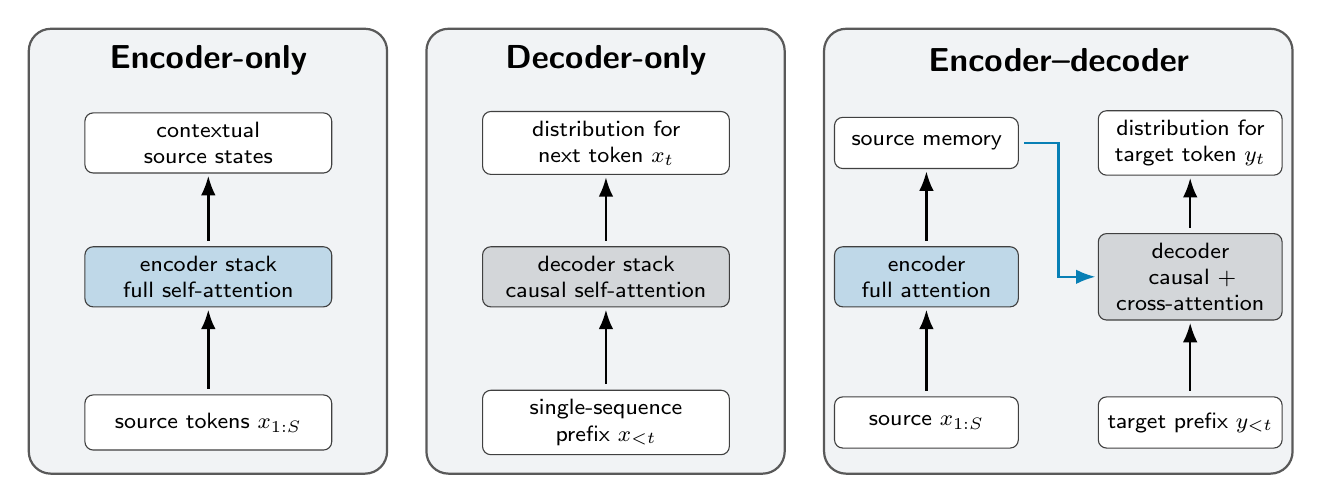
\begin{tikzpicture}[
  typepanel/.style={draw=black!65,rounded corners=8pt,fill=diagramshell,
    line width=0.8pt},
  typebox/.style={draw=black!75,rounded corners=3pt,fill=white,
    text width=29mm,minimum height=7mm,align=center,font=\sffamily\footnotesize},
  typesmall/.style={typebox,text width=21mm,minimum height=6.5mm},
  typeflow/.style={->,>=Latex,line width=0.9pt,shorten <=2pt,
    shorten >=0.8pt},
  typetitle/.style={font=\sffamily\bfseries\large}
]
  \filldraw[typepanel] (0,0) rectangle (4.55,5.65);
  \node[typetitle] at (2.28,5.25) {Encoder-only};
  \node[typebox] (encin) at (2.28,0.65) {source tokens $x_{1:S}$};
  \node[typebox,fill=diagramgpt] (encstack) at (2.28,2.50)
    {encoder stack\\full self-attention};
  \node[typebox] (encout) at (2.28,4.20) {contextual source states};
  \draw[typeflow] (encin) -- (encstack);
  \draw[typeflow] (encstack) -- (encout);

  \begin{scope}[xshift=5.05cm]
    \filldraw[typepanel] (0,0) rectangle (4.55,5.65);
    \node[typetitle] at (2.28,5.25) {Decoder-only};
    \node[typebox] (decin) at (2.28,0.65) {single-sequence prefix $x_{<t}$};
    \node[typebox,fill=white!45!diagramllama] (decstack) at (2.28,2.50)
      {decoder stack\\causal self-attention};
    \node[typebox] (decout) at (2.28,4.20)
      {distribution for next token $x_t$};
    \draw[typeflow] (decin) -- (decstack);
    \draw[typeflow] (decstack) -- (decout);
  \end{scope}

  \begin{scope}[xshift=10.10cm]
    \filldraw[typepanel] (0,0) rectangle (5.95,5.65);
    \node[typetitle] at (2.98,5.25) {Encoder--decoder};
    \node[typesmall] (srcin) at (1.30,0.65) {source $x_{1:S}$};
    \node[typesmall,fill=diagramgpt] (srcenc) at (1.30,2.50)
      {encoder\\full attention};
    \node[typesmall] (memory) at (1.30,4.20) {source memory};
    \node[typesmall] (tgtin) at (4.65,0.65) {target prefix $y_{<t}$};
    \node[typesmall,fill=white!45!diagramllama] (tgtdec) at (4.65,2.50)
      {decoder\\causal + cross-attention};
    \node[typesmall] (tgtout) at (4.65,4.20)
      {distribution for target token $y_t$};
    \draw[typeflow] (srcin) -- (srcenc);
    \draw[typeflow] (srcenc) -- (memory);
    \draw[typeflow] (tgtin) -- (tgtdec);
    \draw[typeflow] (tgtdec) -- (tgtout);
    \coordinate (crosschannel) at ($(memory.east)!0.5!(tgtdec.west)$);
    \draw[typeflow,diagramaccent] (memory.east)
      -- (crosschannel |- memory.east) |- (tgtdec.west);
  \end{scope}
\end{tikzpicture}%
}
\caption{Information flow in three transformer architecture types.
Encoder-only models contextualize a fixed input. Decoder-only models predict
the continuation of one causal sequence. Encoder--decoder models first encode
the complete source and then generate a target that can attend to that source
memory.}
\label{fig:transformer-types}
\end{figure}

\paragraph{Encoder-only.}
An encoder-only model constructs a contextual representation of a fixed input.
Write $\mathcal B^{\rm enc}_{\ell,M}=\mathcal B_{\theta^{\rm enc}_\ell,M}$
for its block at depth $\ell$, with parameters $\theta^{\rm enc}_\ell$.
Let $M_{\rm full}=0$ allow every position to attend to every other position.
The encoder stack is
\begin{equation}
E^0=\operatorname{Embed}_{\rm src}(x_{1:S}),
\qquad
E^{\ell+1}=\mathcal B^{\rm enc}_{\ell,M_{\rm full}}(E^\ell),
\quad \ell=0,\ldots,L_E-1.
\label{eq:encoder-stack}
\end{equation}
Thus every row of $E^{L_E}\in\R^{S\times d}$ can contain information from the
entire source sequence. A task-specific readout converts these contextual
states into predictions.

\paragraph{Decoder-only.}
A decoder-only model represents a single sequence and predicts its
continuation. Similarly,
$\mathcal B^{\rm dec}_{\ell,M}=\mathcal B_{\theta^{\rm dec}_\ell,M}$ denotes
its independently parameterized block at depth $\ell$.
With the triangular mask $M_{\rm causal}$ in \eqref{eq:causal-mask},
\begin{equation}
H^0=\operatorname{Embed}(x_{1:T}),
\qquad
H^{\ell+1}=\mathcal B^{\rm dec}_{\ell,M_{\rm causal}}(H^\ell),
\quad \ell=0,\ldots,L-1.
\label{eq:decoder-only-stack}
\end{equation}
At every depth, the state at position $i$ depends only on tokens at positions
$[i]$. A prompt and its continuation therefore occupy one causal token
stream.

\paragraph{Encoder--decoder.}
An encoder--decoder model is designed for generating a target sequence
conditioned on a separately supplied source sequence. The encoder first
computes $E^{L_E}$ using \eqref{eq:encoder-stack}. This matrix is the
\emph{source memory}: it contains one contextual state for each source
position and remains fixed while the target is generated. The target decoder
starts from
\begin{equation}
D^0=\operatorname{Embed}_{\rm tgt}(y_{<t}).
\end{equation}

For the target decoder, fix each component's parameters at depth $r$ and
abbreviate
$\operatorname{SelfAttn}^r_M=\operatorname{SelfAttn}_{\xi^{\rm self}_r,M}$ and
$\operatorname{FF}^r=\operatorname{FF}_{\psi_r}$.
The map $\operatorname{SelfAttn}^r_M$ is the multi-head self-attention map defined
in \eqref{eq:self-attention-map}; it forms queries, keys, and values from the
same matrix $U$ and applies mask $M$. The map $\operatorname{FF}^r$ is computed
by the positionwise FFN at depth $r$; \eqref{eq:feed-forward-map} gives the
two-layer MLP example.

\emph{Cross-attention} lets each target position retrieve relevant information
from the source memory. For target states $U\in\R^{m\times d}$ and source
memory $E\in\R^{S\times d}$, form queries $Q$ from $U$, and keys $K$ and
values $V$ from $E$. With learned projections
$W^Q,W^K,W^V\in\R^{d\times d_h}$, the same score, softmax, and retrieval
operations as in self-attention give weights $A$ and outputs $O$:
\begin{equation}
\begin{aligned}
Q&=UW^Q,
&K&=EW^K,
&V&=EW^V,\\
A&=\softmax_{\rm row}\!\left(\frac{QK^\top}{\sqrt{d_h}}\right),
&O&=AV.
\end{aligned}
\label{eq:cross-attention-head}
\end{equation}
Here $A\in\R^{m\times S}$ and $O\in\R^{m\times d_h}$.
The map $\operatorname{CrossAttn}^r(U,E)$ combines several such heads,
with separate parameters, by concatenation and an output projection as in
\eqref{eq:self-attention-map}. Its superscript identifies the fixed collection
of cross-attention parameters at depth $r$, separate from $\xi^{\rm self}_r$
and $\psi_r$. Write $N_{r,j}=N_{\nu_{r,j}}$ for the three positionwise
normalization maps, $j\in\{1,2,3\}$, each with its own learned parameters.
These parameter collections may differ between depths.
The decoder block at depth $r$ first mixes information among available
target-prefix positions, producing states $G^r$:
\begin{align}
G^r
&=D^r+\operatorname{SelfAttn}^r_{M_{\rm causal}}
  \bigl(N_{r,1}(D^r)\bigr).
\nonumber\\
\intertext{Cross-attention then enriches these states with information from
the source memory, producing $J^r$:}
J^r
&=G^r+\operatorname{CrossAttn}^r
  \bigl(N_{r,2}(G^r),E^{L_E}\bigr).
\nonumber\\
\intertext{Finally, the FFN transforms the features at each target position
independently, giving the next layer's states $D^{r+1}$:}
D^{r+1}
&=J^r+\operatorname{FF}^r
  \bigl(N_{r,3}(J^r)\bigr).
\label{eq:encoder-decoder-block}
\end{align}
Each step normalizes the input to its sublayer and adds the result back
through a residual connection.

\paragraph{What changes computationally?}
For a length-$n$ sequence, the number of permitted query--key pairs is
$N_{\rm full}(n)$ for one full-attention head and $N_{\rm causal}(n)$ for
one causal head. Count all pairs for the former and only lower-triangular
pairs for the latter:
\begin{equation}
N_{\rm full}(n)=n^2,
\qquad
N_{\rm causal}(n)=\frac{n(n+1)}2.
\label{eq:full-causal-score-count}
\end{equation}
A triangular attention kernel can avoid computing the masked upper triangle.
These expressions count attention pairs per head; they do not include linear
projections or FFN computation.

For source length $S$ and target length $T$, add the pairs used by source
self-attention, causal target self-attention, and target-to-source
cross-attention. With $L_E$ encoder blocks and $L_D$ encoder--decoder blocks,
the total per head is
\begin{equation}
N_{\rm enc\text{-}dec}
=L_ES^2+L_D\frac{T(T+1)}2+L_DST.
\label{eq:encoder-decoder-score-count}
\end{equation}
A fully causal decoder-only
stack of $L$ blocks on a concatenated source and target permits
\begin{equation}
N_{\rm dec\text{-}only}
=L\frac{(S+T)(S+T+1)}2.
\label{eq:decoder-only-score-count}
\end{equation}
Complete runtime comparisons also depend on model depths, widths, head counts,
parameter counts, FFN architectures, and the available hardware kernels.

\begin{remark}[Why are decoder-only models common for language modeling?]
\label{rem:decoder-only-language-modeling}
Next-token pretraining on raw text supplies a prediction target at every
position and requires no separate source--target split. Training and generation
also use the same single-sequence interface. These properties simplify
large-scale training and serving. Encoder--decoder models provide a different
advantage for conditional generation: every target token can use a
bidirectionally encoded source.
\end{remark}

\paragraph{Generation and caching.}
During encoder--decoder generation, the encoder computes the source memory once.
Each decoder layer caches the key and value projections of that fixed memory
for cross-attention. It separately grows a causal self-attention cache for the
generated target. At step $t$, the model forms new queries for the current
target position and reuses both caches.

\section{Take-home messages}

\begin{itemize}[leftmargin=*]
\item A deployed AI system places the language model inside a
``harness'' that constructs context, can maintain state and invoke tools, and
may make repeated model calls.
\item A lossless tokenizer segments a sequence over a base alphabet into
nonempty vocabulary strings. Its token sequence cannot be longer than the
base-symbol sequence and is shorter whenever a selected token contains several
base symbols. Tokens may lack semantic meaning.
\item A probabilistic sequence model maps each finite token prefix to a
next-token distribution. Repeated sampling defines a stochastic process;
finite-sequence probabilities are products of the next-token conditionals.
\item Our archetypical decoder transformer composes embedding, decoder
blocks, and a readout. Each block combines causal attention, a positionwise
FFN, and normalization maps through residual additions.
LayerNorm and RMSNorm are examples of the normalization component.
\item Absolute position embeddings are added once at the input. RoPE and
relative-position biases instead modify the attention calculation in every
layer that uses them.
\item The learned conditional distribution and the decoding algorithm are
different objects. An argmax is optimal for a single zero--one-loss decision.
Repeated tokenwise argmax generally fails to optimize a sequence-level
objective and is a poor default for open-ended generation.
\item A full dense-attention pass on a length-$t$ prefix has quadratic
arithmetic cost. An implementation of causal attention can skip nearly half
the attention pairs used by bidirectional attention at the same length. During
sequential generation, earlier keys and values remain unchanged and are
cached. Each new query uses those rows plus the new key and value. For a
fixed-length initial prompt, this changes total attention work from cubic
to quadratic in the generated length. Old queries have no future use.
\item Maximum context length is an input-capacity limit. Performance on some
retrieval and reasoning tasks may deteriorate before the input reaches this
limit. With bounded attention scores, a single softmax head cannot remain
sharply concentrated as the context grows.
\item The parameter vector $\theta$ contains the learned weights of the
conditional model. The current activations, KV cache, tokenizer, decoding rule,
and harness lie outside $\theta$. Lecture~2 takes up the question of why
learning can produce useful values of $\theta$.
\item Algorithmic properties and engineering viability are separate criteria.
A method with a stronger abstract guarantee may map poorly to available
hardware, while a method with efficient and mature implementations may receive
more development and become difficult to displace.
\end{itemize}

\printendnotes

\section*{Bibliographical notes}
\phantomsection

The compiler analogy is literal at the level of the interface: a lexer maps a
character stream into tokens. A programming-language specification determines
compiler tokens; corpus frequencies help determine LLM tokens. See
\citet{aho2006}. The supplementary appendix describes the BPE construction of
\citet{sennrich2016}, the unigram formulation of \citet{kudo2018}, and the
SentencePiece system of \citet{kudorichardson2018}.

The transformer architecture was introduced by \citet{vaswani2017}. Their
model combined encoder and decoder stacks; the equations in this lecture are a
causal decoder specialization and use a pre-normalized block.
Their Section~3.2.1 motivates the $1/\sqrt{d_h}$ attention-score scaling by
the variance of a query--key dot product.
\Cref{rem:attention-scaling} supplies an explicit random-initialization model
for that calculation.

The SwiGLU FFN architecture was introduced by \citet{shazeer2020}. It uses
two hidden projections and coordinatewise gating; the paper also explains how
to adjust the hidden width when comparing its parameter and operation counts
with a two-layer MLP. SwiGLU is used, for example,
in the Llama~3 architecture \citep{grattafiori2024}.

Three early pretraining recipes made the architectural alternatives concrete.
The original GPT work paired a causal decoder language model with
task-specific supervised fine-tuning \citep{radford2018}. BERT instead
pretrained a bidirectional encoder with a masked-token objective and then
fine-tuned its representations \citep{devlin2019}. T5 retained the
encoder--decoder architecture and expressed many tasks through one text-to-text
interface \citep{raffel2020}. GPT-3 later demonstrated that a sufficiently
large causal language model could use task descriptions and examples supplied
in its context, without a gradient update at test time \citep{brown2020}.
These are historically important successful recipes.

The modular definitions in \Cref{app:transformer-arrangements} follow
the encoder--decoder construction of \citet{vaswani2017} and the architectural
comparisons of \citet{raffel2020}. The latter explain why parameter count and
computation cannot both be matched by changing depth alone and report the
strongest performance from an encoder--decoder model at approximately matched
computation in their setting.

Recent publicly released model families usually preserve the causal
decoder-only interface while changing the surrounding recipe and internal
details. Llama~3 is a dense example \citep{grattafiori2024}, Mistral~7B uses
grouped-query and sliding-window attention \citep{jiang2023}, and DeepSeek-V3
uses a mixture-of-experts architecture \citep{deepseek2024}. The term
\emph{open-weight} asserts release of the numerical weights; training data,
code, and licensing freedoms require separate verification.
For a maintained visual catalogue of model-level architecture diagrams,
configuration links, and compact fact sheets, see the LLM Architecture Gallery
of \citet{raschka2026gallery}.
Figures~\ref{fig:gpt2xl} and~\ref{fig:llama3} are independent LaTeX
renderings of the architectures and dimensions catalogued there; the
Llama~3 specifications were also checked against \citet{grattafiori2024}.

The original paper used additive sinusoidal position vectors. Rotary position embeddings
are due to \citet{su2021}; their position-dependent rotations of queries and
keys expose relative displacement in the attention score.
\Cref{eq:rope-frequencies} gives their fixed geometric frequency schedule.
The bucketed learned
relative-position bias in \eqref{eq:relative-position-bias} follows
\citet{raffel2020}. \citet{press2022} propose ALiBi, which instead adds a fixed
head-dependent linear penalty based on relative distance.

\citet{shazeer2019} identified KV-cache bandwidth as a decoding bottleneck and
introduced multi-query attention: multiple query heads share the same key and
value heads. This reduces cached key--value data and the traffic required to
read it. Grouped-query attention, introduced by \citet{ainslie2023}, provides
an intermediate degree of sharing.

\citet{dao2022} introduced FlashAttention, which computes exact dense
attention by tiling and an online softmax. This reduces memory traffic and
avoids materializing the full attention matrix while retaining the quadratic
arithmetic of exact dense attention. The course returns to this
distinction in Lecture~27.

The bounded-score calculation in \cref{ex:bounded-attention} is elementary.
\citet{chiang2022} study a related length-dependent loss of confidence and show
that the obstruction depends on architectural details; one of their remedies
scales attention logits with $\log T$. This is useful context for the exercise
result.

On the empirical capabilities of trained models across context-window lengths
and locations of relevant information, \citet{liu2024} vary the position of
relevant information in multi-document question answering and key--value
retrieval, demonstrating the distinction between accepting a long context and
using it reliably.
\citet{hong2025} use the term ``context rot'' for performance degradation as
input length grows across a broader collection of tasks and models.

One way to study the division of work described in
\cref{sec:composing-attention} is to write sequence computations as programs
with explicit selection, aggregation, and positionwise operations.
\citet{weiss2021} introduced the \emph{Restricted Access Sequence Processing}
(RASP) language for this purpose, relating its programs to transformer heads
and layers while abstracting away their implementation with weights and
activations. \citet{zhou2024} introduced RASP-L for causal decoder-only
transformers and proposed short-program length as an empirical predictor of
algorithmic learnability and length generalization.
The \hyperref[app:experimental-codebases]{codebases below} support
experiments with these languages.

\citet{arthur1989} studies competing technologies whose benefits increase
with adoption. His model shows how early advantages can lead to technological
lock-in. It provides a framework for the closing discussion of coevolution;
that discussion's application to AI research is a qualitative analogy.

For an analysis of how trained models use RoPE, see \citet{barbero2025}.
Their study of Gemma~7B identifies heads with positional attention patterns,
including attention to the preceding token, and examines how slowly rotating
coordinates support content-based comparisons. They also discuss limitations
of these behaviors when extending context length. This connects the rotation
calculation in \cref{ex:rope} to mechanisms observed in a trained model.
For the exercise's uniform-addressing task, independently uniform frequencies
give a separation guarantee. For language modeling, a geometric schedule
seems a more promising starting point because it deliberately supplies slow
rotations for stable content comparisons. This is a task-dependent judgment,
not a conclusion from a head-to-head empirical comparison of the schedules.

Hoeffding's inequality (\cref{thm:hoeffding}) bounds deviations of sums of
independent bounded random variables \citep{hoeffding1963}. Applying it to independent
random rotation frequencies gives a probabilistic construction of relative
addresses with uniformly separated scores over a prescribed finite context.

\subsection*{Codebases for experiments}
\phantomsection
\label{app:experimental-codebases}

The following codebases support experiments with the constructions in these notes.
\begin{description}[style=nextline,leftmargin=1.5em,labelindent=0pt]
\item[NumPy RASP-L]
A small reference implementation for writing and testing causal RASP-L
sequence programs: \url{https://github.com/apple/ml-np-rasp}.
\item[RASP and Tracr]
The original RASP interpreter displays selectors and intermediate sequence
operations. Tracr compiles a subset of RASP into concrete transformer weights:
\url{https://github.com/tech-srl/RASP} and
\url{https://github.com/google-deepmind/tracr}.
\item[nanochat]
A compact end-to-end codebase containing tokenization, pretraining,
fine-tuning, evaluation, and inference. It includes small CPU and
Apple-Silicon configurations, although training a capable language model still
requires substantial computation: \url{https://github.com/karpathy/nanochat}.
\item[Hugging Face Transformers]
A broad model-definition and checkpoint ecosystem, useful for loading models
and comparing tokenizers, architectures, and generation rules:
\url{https://github.com/huggingface/transformers}.
\item[TransformerLens]
An inspection library for GPT-style models, useful for recording activations
and attention patterns or intervening inside a forward pass:
\url{https://github.com/TransformerLensOrg/TransformerLens}.
\item[llama.cpp]
A local inference implementation that makes tokenization, quantization,
decoding, and key--value-cache behavior accessible to experiments:
\url{https://github.com/ggml-org/llama.cpp}.
\end{description}






\clearpage

\section*{Glossary}

\begin{description}[style=nextline,leftmargin=1.5em,labelindent=0pt]
\item[Harness]
The surrounding program that constructs model inputs, calls the model,
interprets outputs, invokes tools, and controls further model calls.
\item[Task state]
Information maintained by the harness between calls, such as conversation
history, tool results, and progress on the task. Only the portion supplied
to the model is visible to that call.
\item[Prompt]
The initial input supplied to a model call. In the text-only setting, it is a
string that tokenization converts into the initial token sequence.
\item[Prefix]
The token sequence $x_{<t}$ conditioning the prediction at position $t$.
During generation, it consists of the tokenized prompt followed by the tokens
generated so far.
\item[Context]
Information available to the model for its current prediction, represented
here by the token prefix. External task state influences the prediction only
through what the harness supplies.
\item[Context window]
The span of tokens available to the model at a prediction step. In the
full-prefix setting of this note, it contains the prompt and the tokens
generated so far, subject to the maximum context length.
\item[Maximum context length]
The supported upper bound on the number of tokens in the context window.
Prompt and generated tokens share this capacity. Accepting a context of this
length does not guarantee effective use of every token.
\item[Base alphabet; vocabulary; token]
The base alphabet $\Sigma$ contains raw symbols, such as bytes. The vocabulary
$\mathcal V=\{v_1,\ldots,v_V\}$ contains token strings over $\Sigma$.
A token is one vocabulary item, represented inside the model by its index
in $[V]$; it need not be a whole word.
\item[Tokenizer; detokenizer]
A tokenizer maps a string to a sequence of vocabulary indices. The
detokenizer maps $(x_1,\ldots,x_T)$ to $v_{x_1}\cdots v_{x_T}$ in the
text-only setup. It undoes lossless tokenization; the reverse composition
need not recover the original token sequence.
\item[Sequence orientation; matrix layout]
In a sequence display, positions run left to right. In the matrices here,
positions are stacked as rows and the columns index coordinates such as
vocabulary items or learned features. Every vector is a column vector; a
matrix row that stores a vector contains its transpose.
\item[Stochastic process]
A jointly distributed collection of random variables $(X_t)$ indexed by
time or sequence position.
\item[Probabilistic sequence model; stochastic sequence model]
A map $p_\theta:[V]^*\to\Delta_V$ assigning a next-token distribution to
each finite token prefix; see \cref{eq:sequence-model}.
\item[Autoregressive model]
A model specified through next-token conditional distributions
$p_\theta(x_t\mid x_{<t})$. The probability of a fixed finite sequence is
their product, as in \cref{eq:autoregressive-factorization}.
\item[Pretraining; post-training; fine-tuning]
Initial large-scale fitting on broad data; the stage of training that follows
pretraining; and continued parameter training from an existing checkpoint. A
post-training pipeline may contain several fine-tuning procedures.
\item[Inference]
Computing predictions with the model parameters held fixed. Inference can
score a supplied sequence as well as support generation.
\item[Generation]
Repeatedly computing a next-token distribution, selecting a token by a
decoding rule, and appending it to the prefix until a stopping rule applies.
\item[Encoder-only; decoder-only; encoder--decoder transformer]
A bidirectional stack that produces contextual representations of an input; a
causal stack that places prompt and continuation in one sequence; and a
two-stack architecture in which a causal decoder separately reads the
representation produced by a bidirectional encoder.
\item[Self-attention]
Attention whose queries, keys, and values are computed from the same sequence
of activations, with a mask specifying which source positions are available.
\item[Cross-attention]
Attention whose queries come from one sequence and whose keys and values
come from another. Here decoder states query the encoder's source states;
see \cref{eq:cross-attention-head}.
\item[Transformer block]
One repeated layer combining attention and a positionwise feed-forward network
with residual connections and normalization. An encoder--decoder's decoder
block also contains cross-attention.
\item[Embedding]
The learned vector assigned to a token: for token $v$, it is
$E^\top e_v\in\R^d$. The same token uses the same input embedding at each
occurrence; subsequent hidden vectors also depend on context.
\item[Logit]
For a binary probability $p\in(0,1)$, the logit is the log-odds
$\operatorname{logit}(p)=\log(p/(1-p))$.
In a multiclass model $p=\softmax(z)$, the real-valued scores $z_v$ are called
logits: their differences satisfy $z_v-z_u=\log(p_v/p_u)$. A common
additive shift of all logits leaves $p$ unchanged. See
\cref{sec:output-readout} and Lecture~3 on logistic and softmax regression.
\item[Softmax]
The map from real scores $z\in\R^V$ to probabilities
$p_v=\softmax(z)_v=e^{z_v}/\sum_{u=1}^V e^{z_u}$.
In attention, the same map normalizes the scores over the available source
positions for each query.
\item[Categorical distribution]
A distribution on finitely many outcomes, represented here by
$p\in[0,1]^V$ with $\sum_{v=1}^V p_v=1$, where $p_v$ is the probability
of token $v$.
\item[Readout; output head]
A map from a hidden representation to output predictions. The
\emph{softmax readout} here is $h\mapsto\softmax(W_Uh+b_U)$: a learned
affine map produces logits, and softmax converts them to token probabilities.
\item[Parameter]
A trainable numerical quantity in $\theta$, such as an embedding, projection
weight, or bias. Its value is held fixed during the inference computations
described here.
\item[Activation; layer-position activation]
An intermediate value computed for the current input, such as a hidden
vector, query, key, or value. The layer-position activation
$h_i^\ell=(H^\ell_{i,:})^\top$ is the hidden vector at position $i$
after layer $\ell$.
\item[Normalization map]
A vector-to-vector map $N_\nu:\R^d\to\R^d$ with learned parameters $\nu$
that adjusts feature scale and may also center features. Its positionwise lift
acts separately at each sequence position. LayerNorm-type maps are examples; see
\cref{eq:normalization-family}.
\item[Layer normalization (LayerNorm)]
Subtracting a vector's coordinate mean and dividing by
$\sqrt{\text{coordinate variance}+\varepsilon}$, then applying learned
coordinatewise scaling and shifting. It acts separately at each sequence
position, across features. This is $N_{1,\gamma,\beta}$ in
\cref{eq:normalization-family}.
\item[Pre-normalized block]
A block that normalizes the input to each attention or FFN
sublayer before applying it. The sublayer output is then added to the
unnormalized residual stream.
\item[Root-mean-square normalization (RMSNorm)]
Dividing $u$ by $\sqrt{d^{-1}\sum_{r=1}^d u_r^2+\varepsilon}$ and applying
learned coordinatewise scaling. It is the choice $N_{0,\gamma,0}$ in
\cref{eq:normalization-family}: centering and the shift are omitted.
\item[Parameter sharing]
Using the same learned parameters across positions and input sequence lengths,
or in different model calls; see \cref{rem:parameter-reuse}.
\item[Teacher forcing]
Training next-token predictions using the observed preceding tokens as
inputs, rather than feeding back the model's own generated tokens.
\item[Backpropagation]
Applying the chain rule backward through the computation graph to compute
derivatives of a loss with respect to parameters and intermediate values.
An optimizer uses the parameter gradients to update the model.
\item[Weight tying]
Sharing the input embedding matrix with the output readout matrix,
$W_U=E$; see \cref{rem:weight-tying}.
\item[Activation function]
A nonlinear scalar function applied coordinatewise within a neural-network
layer, such as ReLU or GELU. This is a function, whereas an activation is a
computed value.
\item[ReLU]
The rectified linear unit, $\operatorname{ReLU}(z)=\max\{0,z\}$.
\item[GELU]
The Gaussian error linear unit, $\operatorname{GELU}(z)=z\Phi(z)$, where
$\Phi$ is the standard normal cumulative distribution function.
\item[SiLU; swish]
The sigmoid linear unit, $\operatorname{SiLU}(z)=z/(1+e^{-z})$.
This is the swish function used in \cref{rem:swiglu}.
\item[SwiGLU]
A gated FFN computing the map
$W_o(\operatorname{SiLU}(W_g r)\odot(W_v r))$. The two input projections
interact by coordinatewise multiplication before the output projection;
see \cref{rem:swiglu}.
\item[Attention head]
A sequence-to-sequence map
$\operatorname{Head}_{\eta,M}:\R^{T\times d}\to\R^{T\times d_h}$.
Its parameters $\eta$, whose number is independent of $T$, specify the query,
key, and value projections;
the mask $M$ specifies available sources. It computes query--key weights
and uses them to combine value vectors; see \cref{fig:attention-head}.
\item[Query; key; value]
The query $q_i$ is computed from an output position's activation. The key
$k_j$ is computed from a source position's activation and is compared with
$q_i$ to score that source. The value $v_j$ is the source vector used in
the attention-weighted sum; its projection is generally distinct from the
key projection.
\item[Attention score]
A real-valued comparison between query $i$ and source $j$, here the scaled
inner product $q_i^\top k_j/\sqrt{d_h}$, possibly modified by positional
rotations or an additive relative-position bias.
\item[Attention weight]
The coefficient $\alpha_{ij}=e^{s_{ij}}/\sum_{r\in S_i}e^{s_{ir}}$ for
an available source $j\in S_i$, and zero for a masked source. Each query's
weights sum to one; see \cref{eq:available-position-attention}.
\item[Causal mask]
The restriction $j\le i$ on sources available to query position $i$.
It is implemented by adding $-\infty$ to future-position scores before
softmax, giving those sources zero attention weight.
\item[Causal dependence]
The property that an activation at position $i$ depends only on input
positions $j\le i$. In this transformer it follows from causal attention
and positionwise operations, and permits reuse of earlier keys and values.
\item[Multi-head attention (MHA)]
Parallel attention heads whose outputs are concatenated and linearly
projected back to the model dimension. In
$\operatorname{SelfAttn}_{\xi,M}$, the learned parameters
$\xi=(\eta_1,\ldots,\eta_h,W^O)$ include each head's projections and the
output projection; $M$ specifies the mask. Standard MHA gives each query
head its own key and value projections; see \cref{eq:self-attention-map}.
\item[Grouped-query attention (GQA); multi-query attention (MQA)]
GQA partitions query heads into groups that share key and value projections
within each group. MQA uses one shared key/value head for all query heads.
Both reduce the key/value data stored and read during cached decoding.
\item[Residual connection; residual stream]
A residual connection adds a sublayer's output to its input, $h\mapsto
h+F(h)$. The residual stream is the sequence of hidden representations
updated by these additions as they pass through the blocks.
\item[Positionwise map; positionwise lift]
The extension of $f:\R^d\to\R^r$ to sequences by applying the same
function independently at every position, with shared parameters:
$(f(H)_{i,:})^\top=f(h_i)$. See \cref{eq:positionwise-lift}.
\item[Multilayer perceptron (MLP)]
A feed-forward neural network composing learned affine maps and
coordinatewise activation functions, such as ReLU or GELU. The example in
\cref{eq:feed-forward-map} has two affine maps with an activation function
between them.
\item[Positionwise feed-forward network (FFN)]
A neural network applied independently to each position's activation vector,
using shared parameters. Feed-forward means that its computation graph has
no directed cycles. Its input--output function is the positionwise map
$\operatorname{FF}_\psi$, with learned parameters $\psi$. An MLP, a gated
network such as SwiGLU, or a mixture of experts can implement this component;
see \cref{sec:positionwise-ffn}.
\item[Mixture of experts (MoE)]
A layer combining expert maps using input-dependent router weights.
In the sparse version here, each position evaluates only a small selected
subset of experts and takes a weighted sum of their outputs.
\item[Absolute position embedding]
A vector assigned to an absolute sequence position and added to its token
embedding. The position vectors may be learned or prescribed, for example
by sinusoidal functions.
\item[Relative-position bias]
A scalar depending on the displacement $i-j$, or a bucket containing it,
added to the query--key score. See \cref{eq:relative-position-bias}.
\item[Rotary position embeddings (RoPE)]
Position-dependent rotations applied to query and key coordinate pairs
before their inner product. The paired rotations introduce dependence on
relative displacement; see \cref{ex:rope}. RoPE does not itself mask sources.
\item[Decoding rule; sampling; greedy decoding]
A decoding rule selects a next token from the predicted distribution.
Sampling draws a random token with those probabilities. Greedy decoding
selects a token with maximum probability, with a rule for breaking ties;
this need not maximize the probability of the complete sequence.
\item[Prefill]
The initial forward pass over all prompt tokens, which computes their keys
and values and the distribution for the first generated token.
\item[Decode step]
An incremental forward pass for a newly appended token, using earlier cached
keys and values to compute the distribution for the next token.
\item[KV cache]
Stored keys and values from earlier positions, separately for each layer
and key/value head. Causal dependence lets later decode steps reuse them
without recomputing the earlier positions; see \cref{sec:attention-cost}.
\item[Attention entropy]
The entropy $\Hent(\alpha)=-\sum_{j=1}^T\alpha_j\log\alpha_j$ of one
query's attention weights, with $0\log0=0$. It ranges from $0$ for all mass
on one source to $\log T$ for uniform weights on $T$ sources.
\item[Lost in the middle]
An observed pattern of worse performance when relevant information is in
the middle of a long input rather than near its beginning or end.
\item[Context rot]
An empirical term for deteriorating task performance as input length grows,
even within the supported context length.
\end{description}

\section{Exercises}

\exerciseinstructions
\setcounter{courseexercise}{0}
% Shared exercise chunk: l1-rope
The following tool may be used in \cref{ex:rope}.
\begin{theorem}[Hoeffding's inequality]
\label{thm:hoeffding}
Let $n\ge1$ be an integer and let $Z_1,\ldots,Z_n$ be independent real
random variables. Suppose $Z_r\in[a_r,b_r]$ almost surely for each $r\in[n]$,
where $a_r<b_r$ are real numbers. For every real $t\ge0$,
\[
\mathbb P\!\left(\sum_{r=1}^n (Z_r-\mathbb E[Z_r])\ge t\right)
\le \exp\!\left(-\frac{2t^2}{\sum_{r=1}^n(b_r-a_r)^2}\right).
\]
\end{theorem}

\begin{exercisechunk}
\item \textbf{Relative addressing with RoPE.}
\label[exercise]{ex:rope}
Can a query request a value at a specified relative offset while leaving the
source keys unchanged? We will construct such queries, identify collisions between
addresses, and examine how additional coordinate pairs help distinguish them.

Let $T\ge2$ and $d_v\ge1$ be integers. Position $j\in[T]$ stores an
arbitrary fixed value $v_j\in\mathbb R^{d_v}$. Every source uses the same
unrotated unit key $k\in\mathbb R^2$. For each integer offset $1\le d<T$,
we seek a unit-length query vector $q(d)\in\mathbb R^2$ that retrieves $v_{i-d}$ at every
query position $i\in[T]$ with $i>d$. Reusing this query at different positions
should implement the same addressing rule, independently of the stored values.
As described earlier, RoPE modifies the attention calculation
by applying position-dependent linear
transformations---specifically, rotations---to the query and key vectors before
taking their inner product.

\begin{enumerate}[(a)]
\item \textbf{Encoding the request.}
For a real angle $\phi$, define
\[
R_\phi=\begin{pmatrix}\cos\phi&-\sin\phi\\\sin\phi&\cos\phi\end{pmatrix}.
\]
Fix an \emph{angular frequency} $\omega>0$ (called simply a \emph{frequency}
below): moving forward one position increases the rotation angle by
$\omega$ radians. RoPE compares the
query at position $i$ with the key at position $j$ using the score
\[
s_{ij}=(R_{i\omega}q(d))^\top(R_{j\omega}k),\qquad i,j\in[T].
\]
\begin{enumerate}[label=(\roman*),leftmargin=*,beginpenalty=10000]
\item Show that $R_\alpha^\top R_\beta=R_{\beta-\alpha}$ for real angles $\alpha,\beta$.
\item Find the unique unit vector $q(d)$ so that $s_{i,i-d}=1$ whenever $i>d$, and derive a formula
for $s_{ij}$. Show that no source has a larger score.
\item Verify that shifting
$i$ and $j$ by the same integer amount leaves the score unchanged whenever
both positions remain in $[T]$.
\end{enumerate}
\item \textbf{From scores to retrieval.}
For the scores constructed in (a), let $\varnothing\ne S_i\subseteq[T]$
be the source positions available to query $i$. At positive real scale
$\lambda$, define the attention weights and output by
\[
a_{ij}(\lambda)=\frac{e^{\lambda s_{ij}}}
{\sum_{r\in S_i}e^{\lambda s_{ir}}},\quad j\in S_i,
\qquad
o_i(\lambda)=\sum_{j\in S_i}a_{ij}(\lambda)v_j\in\mathbb R^{d_v}.
\]
Fix $\varepsilon\in(0,1/2)$.
\begin{enumerate}[label=(\roman*),leftmargin=*,beginpenalty=10000]
\item For any $j\in S_i$, show that
\[
\|o_i(\lambda)-v_j\|_2
\le (1-a_{ij}(\lambda))\max_{r\in S_i}\|v_r-v_j\|_2.
\]
Thus $a_{ij}(\lambda)>1-\varepsilon$ gives an $O(\varepsilon)$ retrieval
error for fixed values. More explicitly, for a positive real bound $B$,
show that $\|v_r\|_2\le B$ for all $r\in S_i$ gives error less than
$2B\varepsilon$.
\item Show that guaranteeing error at most $2B\varepsilon$
for every such collection of values requires $a_{ij}(\lambda)\ge1-\varepsilon$.

\item Use $S_i=[i]$ and suppose $0<\omega<2\pi/T$.
Show that $i-d$ is the unique maximizing source at every query position
$i>d$. For each such $i$, show that $\lim_{\lambda\to\infty}o_i(\lambda)=v_{i-d}$,
accounting for the weight at every source position.
\item At any such position, prove that $a_{i,i-d}(\lambda)\ge1-\varepsilon$
requires
\[
\lambda\ge\frac{T^2}{2\pi^2}\log\frac{1-\varepsilon}{\varepsilon}.
\]
\end{enumerate}
Hence, for fixed $\varepsilon$, uniform retrieval over values of norm at most
$B$ requires $\lambda=\Omega(T^2)$ in this construction.
Reducing the frequency makes neighboring scores increasingly close; increasing
$\lambda$ compensates for this shrinking gap. The next part examines collisions
when the frequency is held fixed as the sequence grows, and how a window removes
them.
\item \textbf{Collisions and a window repair.}
For this part, hold $d$ fixed and allow the sequence length $T$ to grow. Choose an integer period $P>d$, set $\omega=2\pi/P$, and use the
query construction from (a) with $S_i=[i]$. A \emph{collision} occurs when
another source has the same score as the requested source $i-d$.
\begin{enumerate}[label=(\roman*),leftmargin=*,beginpenalty=10000]
\item Characterize all colliding source positions.
\item Find the first query position
$i>d$ at which a collision occurs.
\item Evaluate $\lim_{\lambda\to\infty}o_i(\lambda)$ at the first collision
position.
\item Now use the window $S_i=\{j\in[i]:i-j<w\}$, where $w$ is a
positive integer. Find the smallest width that retains $i-d$. For this width,
prove that $i-d$ is the unique maximizing source and that
$\lim_{\lambda\to\infty}o_i(\lambda)=v_{i-d}$ for every $i>d$, however long
the sequence becomes.
\end{enumerate}
\item \textbf{Reliable addressing at a fixed score scale.}
Close scores can require high numerical precision to distinguish, even when
$\lambda$ is large. Can additional coordinate pairs create better-separated
scores and permit a smaller scale? Increasing $\lambda$ is equivalent to
increasing query and key norms. To compare this with increasing width, we fix
$\lambda=1$ and unit query and key norms within each pair.

Fix an integer context length $T\ge2$. Throughout this part, use $S_i=[i]$.
Determine, up to constant factors, how many coordinates are necessary and
sufficient to give the requested
source attention weight at least $3/4$, simultaneously for every integer
offset $1\le d<T$ and every query position $i\in[T]$ with $i>d$.

Let $m$ be a positive integer, which determines the number of coordinate pairs used.
For each coordinate pair $r\in[m]$, use a
fixed unit key $k_r\in\mathbb R^2$, a frequency $\omega_r\in[0,2\pi)$,
and the unit query $q_r(d)\in\mathbb R^2$ constructed in (a).
Define the combined score as
\[
s_{ij}=\sum_{r=1}^m
(R_{i\omega_r}q_r(d))^\top(R_{j\omega_r}k_r),\qquad i,j\in[T].
\]
\begin{enumerate}[label=(\roman*),leftmargin=*,beginpenalty=10000]
\item \textbf{A necessary dimension.}
Show that all scores lie in $[-m,m]$. Use \cref{ex:bounded-attention} to prove
that, at query position $i=T$, attention weight at least $3/4$ on the requested
source requires
\[
m\ge\tfrac12\log\bigl(3(T-1)\bigr).
\]
\item \textbf{Finding frequencies that separate addresses.}
Prove that, for every integer $m\ge8\log(2T)$, there exist frequencies
$\omega_1,\ldots,\omega_m\in[0,2\pi)$ such that
\begin{equation}
\label{eq:rope-separated-addresses}
\sum_{r=1}^m\cos(\omega_r h)\le m/2
\quad\text{for every integer }h\text{ with }1\le|h|<T.
\end{equation}
\item \textbf{Retrieval at every position and offset.}
Fix frequencies satisfying \cref{eq:rope-separated-addresses}. Show that the requested source has score
$m$ and that every other available source has score at most $m/2$,
simultaneously for all offsets and query positions in the question.
Prove that the total attention weight outside the requested source is at most
$(T-1)e^{-m/2}$. Deduce that
$m=\lceil8\log(2T)\rceil$ suffices for target weight at least $3/4$ with
$\lambda=1$. State the resulting error bound when every value vector has
norm at most a positive real bound $B$. Together with (i), conclude that
$\Theta(\log T)$ coordinate pairs are necessary and sufficient.
\end{enumerate}

\end{enumerate}

\paragraph{Conclusion.}
With suitably chosen frequencies, RoPE supports relative addressing with
logarithmic width and bounded coordinates. Extra coordinate pairs both
distinguish addresses and accumulate
the score advantage needed to concentrate attention
(\cref{ex:bounded-attention}). Keeping each coordinate bounded still allows
the total score to grow: width supplies an alternative to increasing $\lambda$.

Standard RoPE instead uses geometrically spaced frequencies to provide both
rapidly and slowly varying positional features. The existence guarantee in
(d) does not automatically apply to that schedule. Indeed, its frequencies
satisfy $0<\omega_r\le1$, so at displacement $h=1$,
\[
\sum_{r=1}^m\cos\omega_r\ge m\cos1>m/2.
\]
Thus it fails the particular sufficient separation condition in (d)(ii);
this does not rule out retrieval with that schedule.

\begin{hints}
For (d)(i), apply the bound from \cref{ex:bounded-attention} with $T$ sources
and score range $2m$.
For (d)(ii), choose the frequencies independently and uniformly on $[0,2\pi)$.
Compute $\mathbb E[\cos(\omega_r h)]$ for a nonzero integer $h$, then apply
\cref{thm:hoeffding} and a union bound over $h\in[T-1]$.
Use the evenness of cosine to handle negative $h$.
\end{hints}
\end{exercisechunk}

% Shared exercise chunk: l1-greedy-decoding
\begin{exercisechunk}
\item \textbf{Greedy decoding and repetition.}
\label[exercise]{ex:greedy-decoding}
A toy language model completes the prefix ``The movie was''.
Let ``\texttt{very}'' and ``\texttt{good.}'' (including the full stop, not including the apostrophes, which we will drop)
be two tokens in the model's output token vocabulary.
Given this prefix, the toy model outputs
token \texttt{very} with probability $0.6$ or
token \texttt{good.}
with probability $0.4$.
When the prefix ends with token
\texttt{very}, it repeats the same
choice; when it ends with \texttt{good.},
it outputs the stop token with probability one and generation stops.
Count the stop token as a generated token, including for the budget below.

\begin{enumerate}[(a)]
\item What token sequence does greedy decoding produce with a budget of $10$
additional tokens? What token sequence does it produce without a budget?
\item Under sampling, calculate the probability that generation terminates
within $10$ additional tokens. Without a token budget, show that generation
terminates with probability one and compute the expected number of generated
tokens.
\item Which complete sentence has the highest probability under the model?
What is its probability?
\end{enumerate}

\paragraph{Connection to language models.}
\href{https://arxiv.org/pdf/1908.04319v2}{Welleck et al. (2019, Table~4,
p.~11)} show a GPT-2 continuation that repeats ``Portuguese'' under greedy
decoding. The
\href{https://huggingface.co/Qwen/Qwen3-8B}{Qwen3-8B model card}
also warns that greedy decoding can cause endless repetition in thinking mode.
\end{exercisechunk}

% Shared exercise chunk: l1-bounded-attention
\begin{exercisechunk}
\item \textbf{Bounded scores and attention concentration.}
\label[exercise]{ex:bounded-attention}
Let $T\ge2$ be an integer and let $a,b\in\mathbb R$ satisfy $a\le b$.
Write $R=b-a$ for the score range. For a score vector $s\in[a,b]^T$,
define the probability vector $\alpha(s)$ by
\[
\alpha_j(s)=\frac{e^{s_j}}{\sum_{r=1}^T e^{s_r}},\qquad j\in[T].
\]
\begin{enumerate}[(a)]
\item
Compute $\sup_{s\in[a,b]^T}\max_{j\in[T]}\alpha_j(s)$ and give a score
vector attaining this value.
\item \emph{Optional extension.}
Writing $H(\alpha)=-\sum_{j=1}^T\alpha_j\log\alpha_j$ for the
\emph{entropy}, show that for every $s\in[a,b]^T$,
\[
\log T-R\le H(\alpha(s))\le\log T.
\]
Deduce that, for fixed $a,b$, $H(\alpha(s))/\log T\to1$ uniformly over
$s\in[a,b]^T$ as $T\to\infty$. This concerns entropy relative to its maximum;
it does not imply $\sum_{j=1}^T|\alpha_j(s)-1/T|\to0$.
\item For a fixed $c\in(0,1)$, determine the smallest $R\ge0$ for which
some $s\in[a,a+R]^T$ satisfies $\max_{j\in[T]}\alpha_j(s)\ge c$.
Give such a score vector at this minimum range.
Describe how this minimum range grows with $T$ for fixed $c$, and deduce
whether a score range independent of $T$ can maintain $\max_j\alpha_j(s)\ge c$
as $T\to\infty$.
\end{enumerate}
\end{exercisechunk}


\clearpage
\appendix
\renewcommand{\thesection}{\Alph{section}}
\section{How tokenizers are constructed}
\label{app:tokenizer-construction}

Two common corpus-based constructions illustrate the main ideas.
\begin{enumerate}[leftmargin=*]
\item \emph{Byte-pair encoding (BPE).} Merging a frequent adjacent pair
shortens the corpus's tokenization wherever that pair is replaced.
Start with base symbols, count adjacent
token pairs in the training corpus, merge a most frequent pair into a new
vocabulary item, and repeat until the desired vocabulary size is reached. The
learned merge order determines the segmentation of new text.
\item \emph{Unigram tokenization.} To compare alternative segmentations,
assign each candidate token string $v$ a probability $q(v)$.
Start with a large collection of candidates and score a segmentation
$x_1,\ldots,x_T$ by multiplying its token probabilities,
or equivalently adding their logarithms:
\begin{equation}
\prod_{t=1}^T q(v_{x_t}),
\qquad\text{or equivalently}\qquad
\sum_{t=1}^T\log q(v_{x_t}).
\end{equation}
Fit the probabilities to the corpus, remove candidates whose deletion hurts
the likelihood least, and repeat. At encoding time one may choose a
highest-scoring segmentation or sample among segmentations.
\end{enumerate}

\clearpage
\begin{thebibliography}{99}
\bibitem[Arthur(1989)]{arthur1989}
W. Brian Arthur.
\newblock Competing Technologies, Increasing Returns, and Lock-In by
Historical Events.
\newblock \emph{The Economic Journal}, 99(394):116--131, 1989.
\newblock \url{https://doi.org/10.2307/2234208}.

\bibitem[Aho et al.(2006)]{aho2006}
A. V. Aho, M. S. Lam, R. Sethi, and J. D. Ullman.
\newblock \emph{Compilers: Principles, Techniques, and Tools}.
\newblock Addison--Wesley, second edition, 2006.

\bibitem[Sennrich et al.(2016)]{sennrich2016}
R. Sennrich, B. Haddow, and A. Birch.
\newblock Neural Machine Translation of Rare Words with Subword Units.
\newblock \emph{ACL}, 2016.
\newblock \url{https://arxiv.org/abs/1508.07909}.

\bibitem[Kudo(2018)]{kudo2018}
T. Kudo.
\newblock Subword Regularization: Improving Neural Network Translation Models
with Multiple Subword Candidates.
\newblock \emph{ACL}, 2018.
\newblock \url{https://arxiv.org/abs/1804.10959}.

\bibitem[Kudo and Richardson(2018)]{kudorichardson2018}
T. Kudo and J. Richardson.
\newblock SentencePiece: A Simple and Language Independent Subword Tokenizer
and Detokenizer for Neural Text Processing.
\newblock \emph{EMNLP System Demonstrations}, 2018.
\newblock \url{https://aclanthology.org/D18-2012/}.

\bibitem[Vaswani et al.(2017)]{vaswani2017}
A. Vaswani, N. Shazeer, N. Parmar, J. Uszkoreit, L. Jones, A. Gomez,
L. Kaiser, and I. Polosukhin.
\newblock Attention Is All You Need.
\newblock \emph{NeurIPS}, 2017.
\newblock \url{https://arxiv.org/abs/1706.03762}.

\bibitem[Radford et al.(2018)]{radford2018}
A. Radford, K. Narasimhan, T. Salimans, and I. Sutskever.
\newblock Improving Language Understanding by Generative Pre-Training.
\newblock OpenAI technical report, 2018.
\newblock \url{https://cdn.openai.com/research-covers/language-unsupervised/language_understanding_paper.pdf}.

\bibitem[Devlin et al.(2019)]{devlin2019}
J. Devlin, M.-W. Chang, K. Lee, and K. Toutanova.
\newblock BERT: Pre-training of Deep Bidirectional Transformers for Language
Understanding.
\newblock \emph{NAACL}, 2019.
\newblock \url{https://arxiv.org/abs/1810.04805}.

\bibitem[Brown et al.(2020)]{brown2020}
T. B. Brown et al.
\newblock Language Models are Few-Shot Learners.
\newblock \emph{NeurIPS}, 2020.
\newblock \url{https://arxiv.org/abs/2005.14165}.

\bibitem[Grattafiori et al.(2024)]{grattafiori2024}
A. Grattafiori et al.
\newblock The Llama 3 Herd of Models.
\newblock 2024.
\newblock \url{https://arxiv.org/abs/2407.21783}.

\bibitem[Raschka(2026)]{raschka2026gallery}
S. Raschka.
\newblock LLM Architecture Gallery.
\newblock Maintained online reference, accessed September 3, 2026.
\newblock \url{https://sebastianraschka.com/llm-architecture-gallery/}.

\bibitem[Jiang et al.(2023)]{jiang2023}
A. Q. Jiang et al.
\newblock Mistral 7B.
\newblock 2023.
\newblock \url{https://arxiv.org/abs/2310.06825}.

\bibitem[DeepSeek-AI(2024)]{deepseek2024}
DeepSeek-AI.
\newblock DeepSeek-V3 Technical Report.
\newblock 2024.
\newblock \url{https://arxiv.org/abs/2412.19437}.

\bibitem[Hoeffding(1963)]{hoeffding1963}
W. Hoeffding.
\newblock Probability Inequalities for Sums of Bounded Random Variables.
\newblock \emph{Journal of the American Statistical Association},
58(301):13--30, 1963.
\newblock \url{https://doi.org/10.1080/01621459.1963.10500830}.

\bibitem[Barbero et al.(2025)]{barbero2025}
F. Barbero, A. Vitvitskyi, C. Perivolaropoulos, R. Pascanu,
and P. Veli\v{c}kovi\'c.
\newblock Round and Round We Go! What Makes Rotary Positional Encodings Useful?
\newblock \emph{ICLR}, 2025.
\newblock \url{https://arxiv.org/abs/2410.06205}.

\bibitem[Su et al.(2021)]{su2021}
J. Su, Y. Lu, S. Pan, A. Murtadha, B. Wen, and Y. Liu.
\newblock RoFormer: Enhanced Transformer with Rotary Position Embedding.
\newblock 2021.
\newblock \url{https://arxiv.org/abs/2104.09864}.

\bibitem[Raffel et al.(2020)]{raffel2020}
C. Raffel, N. Shazeer, A. Roberts, K. Lee, S. Narang, M. Matena,
Y. Zhou, W. Li, and P. J. Liu.
\newblock Exploring the Limits of Transfer Learning with a Unified
Text-to-Text Transformer.
\newblock \emph{Journal of Machine Learning Research}, 21(140):1--67, 2020.
\newblock \url{https://www.jmlr.org/papers/v21/20-074.html}.

\bibitem[Press et al.(2022)]{press2022}
O. Press, N. A. Smith, and M. Lewis.
\newblock Train Short, Test Long: Attention with Linear Biases Enables Input
Length Extrapolation.
\newblock \emph{ICLR}, 2022.
\newblock \url{https://arxiv.org/abs/2108.12409}.

\bibitem[Shazeer(2019)]{shazeer2019}
N. Shazeer.
\newblock Fast Transformer Decoding: One Write-Head is All You Need.
\newblock 2019.
\newblock \url{https://arxiv.org/abs/1911.02150}.

\bibitem[Shazeer(2020)]{shazeer2020}
N. Shazeer.
\newblock GLU Variants Improve Transformer.
\newblock 2020.
\newblock \url{https://arxiv.org/abs/2002.05202}.

\bibitem[Ainslie et al.(2023)]{ainslie2023}
J. Ainslie, J. Lee-Thorp, M. de Jong, Y. Zemlyanskiy, F. Lebr\'on,
and S. Sanghai.
\newblock GQA: Training Generalized Multi-Query Transformer Models from
Multi-Head Checkpoints.
\newblock \emph{EMNLP}, 2023.
\newblock \url{https://arxiv.org/abs/2305.13245}.

\bibitem[Dao et al.(2022)]{dao2022}
T. Dao, D. Y. Fu, S. Ermon, A. Rudra, and C. R\'e.
\newblock FlashAttention: Fast and Memory-Efficient Exact Attention with
IO-Awareness.
\newblock \emph{NeurIPS}, 2022.
\newblock \url{https://arxiv.org/abs/2205.14135}.

\bibitem[Chiang and Cholak(2022)]{chiang2022}
D. Chiang and P. Cholak.
\newblock Overcoming a Theoretical Limitation of Self-Attention.
\newblock \emph{ACL}, 2022.
\newblock \url{https://aclanthology.org/2022.acl-long.527/}.

\bibitem[Liu et al.(2024)]{liu2024}
N. F. Liu, K. Lin, J. Hewitt, A. Paranjape, M. Bevilacqua, F. Petroni,
and P. Liang.
\newblock Lost in the Middle: How Language Models Use Long Contexts.
\newblock \emph{Transactions of the Association for Computational
Linguistics}, 2024.
\newblock \url{https://arxiv.org/abs/2307.03172}.

\bibitem[Hong et al.(2025)]{hong2025}
K. Hong, A. Troynikov, and J. Huber.
\newblock Context Rot: How Increasing Input Tokens Impacts LLM Performance.
\newblock Chroma technical report, 2025.
\newblock \url{https://www.trychroma.com/research/context-rot}.

\bibitem[Weiss et al.(2021)]{weiss2021}
G. Weiss, Y. Goldberg, and E. Yahav.
\newblock Thinking Like Transformers.
\newblock \emph{ICML}, 2021.
\newblock \url{https://proceedings.mlr.press/v139/weiss21a.html}.

\bibitem[Zhou et al.(2024)]{zhou2024}
H. Zhou, A. Bradley, E. Littwin, N. Razin, O. Saremi, J. Susskind,
S. Bengio, and P. Nakkiran.
\newblock What Algorithms Can Transformers Learn? A Study in Length
Generalization.
\newblock \emph{ICLR}, 2024.
\newblock \url{https://arxiv.org/abs/2310.16028}.
\end{thebibliography}

\end{document}
